\documentclass[1p]{elsarticle_modified}
%\bibliographystyle{elsarticle-num}

%\usepackage[colorlinks]{hyperref}
%\usepackage{abbrmath_seonhwa} %\Abb, \Ascr, \Acal ,\Abf, \Afrak
\usepackage{amsfonts}
\usepackage{amssymb}
\usepackage{amsmath}
\usepackage{amsthm}
\usepackage{scalefnt}
\usepackage{amsbsy}
\usepackage{kotex}
\usepackage{caption}
\usepackage{subfig}
\usepackage{color}
\usepackage{graphicx}
\usepackage{xcolor} %% white, black, red, green, blue, cyan, magenta, yellow
\usepackage{float}
\usepackage{setspace}
\usepackage{hyperref}

\usepackage{tikz}
\usetikzlibrary{arrows}

\usepackage{multirow}
\usepackage{array} % fixed length table
\usepackage{hhline}

%%%%%%%%%%%%%%%%%%%%%
\makeatletter
\renewcommand*\env@matrix[1][\arraystretch]{%
	\edef\arraystretch{#1}%
	\hskip -\arraycolsep
	\let\@ifnextchar\new@ifnextchar
	\array{*\c@MaxMatrixCols c}}
\makeatother %https://tex.stackexchange.com/questions/14071/how-can-i-increase-the-line-spacing-in-a-matrix
%%%%%%%%%%%%%%%

\usepackage[normalem]{ulem}

\newcommand{\msout}[1]{\ifmmode\text{\sout{\ensuremath{#1}}}\else\sout{#1}\fi}
%SOURCE: \msout is \stkout macro in https://tex.stackexchange.com/questions/20609/strikeout-in-math-mode

\newcommand{\cancel}[1]{
	\ifmmode
	{\color{red}\msout{#1}}
	\else
	{\color{red}\sout{#1}}
	\fi
}

\newcommand{\add}[1]{
	{\color{blue}\uwave{#1}}
}

\newcommand{\replace}[2]{
	\ifmmode
	{\color{red}\msout{#1}}{\color{blue}\uwave{#2}}
	\else
	{\color{red}\sout{#1}}{\color{blue}\uwave{#2}}
	\fi
}

\newcommand{\Sol}{\mathcal{S}} %segment
\newcommand{\D}{D} %diagram
\newcommand{\A}{\mathcal{A}} %arc


%%%%%%%%%%%%%%%%%%%%%%%%%%%%%5 test

\def\sl{\operatorname{\textup{SL}}(2,\Cbb)}
\def\psl{\operatorname{\textup{PSL}}(2,\Cbb)}
\def\quan{\mkern 1mu \triangleright \mkern 1mu}

\theoremstyle{definition}
\newtheorem{thm}{Theorem}[section]
\newtheorem{prop}[thm]{Proposition}
\newtheorem{lem}[thm]{Lemma}
\newtheorem{ques}[thm]{Question}
\newtheorem{cor}[thm]{Corollary}
\newtheorem{defn}[thm]{Definition}
\newtheorem{exam}[thm]{Example}
\newtheorem{rmk}[thm]{Remark}
\newtheorem{alg}[thm]{Algorithm}

\newcommand{\I}{\sqrt{-1}}
\begin{document}

%\begin{frontmatter}
%
%\title{Boundary parabolic representations of knots up to 8 crossings}
%
%%% Group authors per affiliation:
%\author{Yunhi Cho} 
%\address{Department of Mathematics, University of Seoul, Seoul, Korea}
%\ead{yhcho@uos.ac.kr}
%
%
%\author{Seonhwa Kim} %\fnref{s_kim}}
%\address{Center for Geometry and Physics, Institute for Basic Science, Pohang, 37673, Korea}
%\ead{ryeona17@ibs.re.kr}
%
%\author{Hyuk Kim}
%\address{Department of Mathematical Sciences, Seoul National University, Seoul 08826, Korea}
%\ead{hyukkim@snu.ac.kr}
%
%\author{Seokbeom Yoon}
%\address{Department of Mathematical Sciences, Seoul National University, Seoul, 08826,  Korea}
%\ead{sbyoon15@snu.ac.kr}
%
%\begin{abstract}
%We find all boundary parabolic representation of knots up to 8 crossings.
%
%\end{abstract}
%\begin{keyword}
%    \MSC[2010] 57M25 
%\end{keyword}
%
%\end{frontmatter}

%\linenumbers
%\tableofcontents
%
\newcommand\colored[1]{\textcolor{white}{\rule[-0.35ex]{0.8em}{1.4ex}}\kern-0.8em\color{red} #1}%
%\newcommand\colored[1]{\textcolor{white}{ #1}\kern-2.17ex	\textcolor{white}{ #1}\kern-1.81ex	\textcolor{white}{ #1}\kern-2.15ex\color{red}#1	}

{\Large $\underline{12a_{0426}~(K12a_{0426})}$}

\setlength{\tabcolsep}{10pt}
\renewcommand{\arraystretch}{1.6}
\vspace{1cm}\begin{tabular}{m{100pt}>{\centering\arraybackslash}m{274pt}}
\multirow{5}{120pt}{
	\centering
	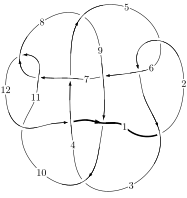
\includegraphics[width=112pt]{../../../GIT/diagram.site/Diagrams/png/1227_12a_0426.png}\\
\ \ \ A knot diagram\footnotemark}&
\allowdisplaybreaks
\textbf{Linearized knot diagam} \\
\cline{2-2}
 &
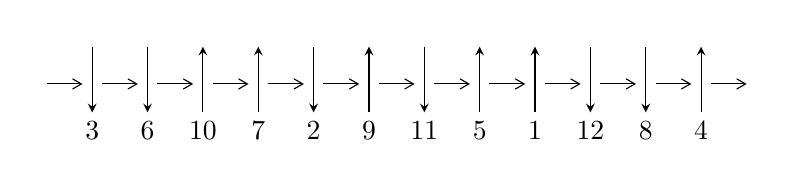
\begin{tikzpicture}[x=20pt, y=17pt]
	% nodes
	\node (C0) at (0, 0) {};
	\node (C1) at (1, 0) {};
	\node (C1U) at (1, +1) {};
	\node (C1D) at (1, -1) {3};

	\node (C2) at (2, 0) {};
	\node (C2U) at (2, +1) {};
	\node (C2D) at (2, -1) {6};

	\node (C3) at (3, 0) {};
	\node (C3U) at (3, +1) {};
	\node (C3D) at (3, -1) {10};

	\node (C4) at (4, 0) {};
	\node (C4U) at (4, +1) {};
	\node (C4D) at (4, -1) {7};

	\node (C5) at (5, 0) {};
	\node (C5U) at (5, +1) {};
	\node (C5D) at (5, -1) {2};

	\node (C6) at (6, 0) {};
	\node (C6U) at (6, +1) {};
	\node (C6D) at (6, -1) {9};

	\node (C7) at (7, 0) {};
	\node (C7U) at (7, +1) {};
	\node (C7D) at (7, -1) {11};

	\node (C8) at (8, 0) {};
	\node (C8U) at (8, +1) {};
	\node (C8D) at (8, -1) {5};

	\node (C9) at (9, 0) {};
	\node (C9U) at (9, +1) {};
	\node (C9D) at (9, -1) {1};

	\node (C10) at (10, 0) {};
	\node (C10U) at (10, +1) {};
	\node (C10D) at (10, -1) {12};

	\node (C11) at (11, 0) {};
	\node (C11U) at (11, +1) {};
	\node (C11D) at (11, -1) {8};

	\node (C12) at (12, 0) {};
	\node (C12U) at (12, +1) {};
	\node (C12D) at (12, -1) {4};
	\node (C13) at (13, 0) {};

	% arrows
	\draw[->,>={angle 60}]
	(C0) edge (C1) (C1) edge (C2) (C2) edge (C3) (C3) edge (C4) (C4) edge (C5) (C5) edge (C6) (C6) edge (C7) (C7) edge (C8) (C8) edge (C9) (C9) edge (C10) (C10) edge (C11) (C11) edge (C12) (C12) edge (C13) ;	\draw[->,>=stealth]
	(C1U) edge (C1D) (C2U) edge (C2D) (C3D) edge (C3U) (C4D) edge (C4U) (C5U) edge (C5D) (C6D) edge (C6U) (C7U) edge (C7D) (C8D) edge (C8U) (C9D) edge (C9U) (C10U) edge (C10D) (C11U) edge (C11D) (C12D) edge (C12U) ;
	\end{tikzpicture} \\
\hhline{~~} \\& 
\textbf{Solving Sequence} \\ \cline{2-2} 
 &
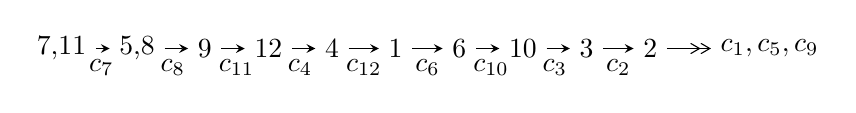
\begin{tikzpicture}[x=23pt, y=7pt]
	% node
	\node (A0) at (-1/8, 0) {7,11};
	\node (A1) at (17/16, 0) {5,8};
	\node (A2) at (17/8, 0) {9};
	\node (A3) at (25/8, 0) {12};
	\node (A4) at (33/8, 0) {4};
	\node (A5) at (41/8, 0) {1};
	\node (A6) at (49/8, 0) {6};
	\node (A7) at (57/8, 0) {10};
	\node (A8) at (65/8, 0) {3};
	\node (A9) at (73/8, 0) {2};
	\node (C1) at (1/2, -1) {$c_{7}$};
	\node (C2) at (13/8, -1) {$c_{8}$};
	\node (C3) at (21/8, -1) {$c_{11}$};
	\node (C4) at (29/8, -1) {$c_{4}$};
	\node (C5) at (37/8, -1) {$c_{12}$};
	\node (C6) at (45/8, -1) {$c_{6}$};
	\node (C7) at (53/8, -1) {$c_{10}$};
	\node (C8) at (61/8, -1) {$c_{3}$};
	\node (C9) at (69/8, -1) {$c_{2}$};
	\node (A10) at (11, 0) {$c_{1},c_{5},c_{9}$};

	% edge
	\draw[->,>=stealth]	
	(A0) edge (A1) (A1) edge (A2) (A2) edge (A3) (A3) edge (A4) (A4) edge (A5) (A5) edge (A6) (A6) edge (A7) (A7) edge (A8) (A8) edge (A9) ;
	\draw[->>,>={angle 60}]	
	(A9) edge (A10);
\end{tikzpicture} \\ 

\end{tabular} \\

\footnotetext{
The image of knot diagram is generated by the software ``\textbf{Draw programme}" developed by Andrew Bartholomew(\url{http://www.layer8.co.uk/maths/draw/index.htm\#Running-draw}), where we modified some parts for our purpose(\url{https://github.com/CATsTAILs/LinksPainter}).
}\phantom \\ \newline 
\centering \textbf{Ideals for irreducible components\footnotemark of $X_{\text{par}}$} 
 
\begin{align*}
I^u_{1}&=\langle 
5 u^{17}-11 u^{16}+\cdots+3 b-11,\;u^{17}+u^{16}+\cdots+2 a+4,\;u^{18}-3 u^{17}+\cdots-6 u+2\rangle \\
I^u_{2}&=\langle 
2.93297\times10^{19} u^{49}-3.08421\times10^{20} u^{48}+\cdots+4.46875\times10^{17} b-5.17754\times10^{20},\\
\phantom{I^u_{2}}&\phantom{= \langle  }-2.95147\times10^{19} u^{49}+6.16285\times10^{20} u^{48}+\cdots+5.80937\times10^{18} a+6.41388\times10^{21},\\
\phantom{I^u_{2}}&\phantom{= \langle  }u^{50}-11 u^{49}+\cdots-165 u+13\rangle \\
I^u_{3}&=\langle 
- u^5 a- u^5+2 u^3 a+u^3-2 a u+b- u+1,\;2 u^4 a+u^3 a-3 u^4-2 u^2 a-2 u^3+a^2-2 a u+u^2+3 u+2,\\
\phantom{I^u_{3}}&\phantom{= \langle  }u^6+u^5- u^4-2 u^3+u+1\rangle \\
I^u_{4}&=\langle 
u^5- u^3+b+u,\;u^3+a,\;u^6+u^5- u^4-2 u^3+u+1\rangle \\
I^u_{5}&=\langle 
-2 u^{43} a-4 u^{42} a+\cdots+4 b-65,\;50 u^{43} a-95 u^{43}+\cdots-468 a+943,\;u^{44}+3 u^{43}+\cdots-14 u-1\rangle \\
I^u_{6}&=\langle 
3 u^{15}+5 u^{14}-4 u^{13}-18 u^{12}-11 u^{11}+4 u^{10}+4 u^9+u^8+21 u^7+32 u^6+22 u^5+9 u^4+10 u^3+5 u^2+b- u-1,\\
\phantom{I^u_{6}}&\phantom{= \langle  }-7 u^{15}-28 u^{14}+\cdots+2 a-22,\;u^{16}+4 u^{15}+\cdots+8 u+2\rangle \\
I^u_{7}&=\langle 
- u^2 a+b-1,\;a^2+2 a u+2 u^2+a+3 u+2,\;u^3+u^2-1\rangle \\
I^u_{8}&=\langle 
- u^3 a- u^2 a- u^3+a u+2 b+1,\;- u^2 a+u^3+a^2+a u-2 u^2+a- u+2,\;u^4- u^2+1\rangle \\
I^u_{9}&=\langle 
-71757 a^7+7931089 b+\cdots-9811314 a+3141666,\\
\phantom{I^u_{9}}&\phantom{= \langle  }a^8+6 a^6-6 a^5+26 a^4-18 a^3+87 a^2-60 a+73,\;u-1\rangle \\
\\
\end{align*}
\raggedright * 9 irreducible components of $\dim_{\mathbb{C}}=0$, with total 212 representations.\\
\footnotetext{All coefficients of polynomials are rational numbers. But the coefficients are sometimes approximated in decimal forms when there is not enough margin.}
\newpage
\renewcommand{\arraystretch}{1}
\centering \section*{I. $I^u_{1}= \langle 5 u^{17}-11 u^{16}+\cdots+3 b-11,\;u^{17}+u^{16}+\cdots+2 a+4,\;u^{18}-3 u^{17}+\cdots-6 u+2 \rangle$}
\flushleft \textbf{(i) Arc colorings}\\
\begin{tabular}{m{7pt} m{180pt} m{7pt} m{180pt} }
\flushright $a_{7}=$&$\begin{pmatrix}1\\0\end{pmatrix}$ \\
\flushright $a_{11}=$&$\begin{pmatrix}0\\u\end{pmatrix}$ \\
\flushright $a_{5}=$&$\begin{pmatrix}-\frac{1}{2} u^{17}-\frac{1}{2} u^{16}+\cdots-\frac{3}{2} u^2-2\\-\frac{5}{3} u^{17}+\frac{11}{3} u^{16}+\cdots-\frac{23}{3} u+\frac{11}{3}\end{pmatrix}$ \\
\flushright $a_{8}=$&$\begin{pmatrix}1\\u^2\end{pmatrix}$ \\
\flushright $a_{9}=$&$\begin{pmatrix}\frac{1}{2} u^{17}-\frac{5}{2} u^{16}+\cdots+5 u-3\\-\frac{5}{3} u^{17}+\frac{11}{3} u^{16}+\cdots-\frac{23}{3} u+\frac{11}{3}\end{pmatrix}$ \\
\flushright $a_{12}=$&$\begin{pmatrix}- u\\- u^3+u\end{pmatrix}$ \\
\flushright $a_{4}=$&$\begin{pmatrix}\frac{7}{6} u^{17}-\frac{25}{6} u^{16}+\cdots+\frac{23}{3} u-\frac{17}{3}\\-\frac{5}{3} u^{17}+\frac{11}{3} u^{16}+\cdots-\frac{23}{3} u+\frac{11}{3}\end{pmatrix}$ \\
\flushright $a_{1}=$&$\begin{pmatrix}\frac{19}{6} u^{17}-\frac{37}{6} u^{16}+\cdots+\frac{32}{3} u-\frac{14}{3}\\-\frac{2}{3} u^{17}+\frac{2}{3} u^{16}+\cdots+\frac{1}{3} u-\frac{1}{3}\end{pmatrix}$ \\
\flushright $a_{6}=$&$\begin{pmatrix}-\frac{7}{6} u^{17}+\frac{25}{6} u^{16}+\cdots-\frac{23}{3} u+\frac{17}{3}\\\frac{2}{3} u^{17}-\frac{2}{3} u^{16}+\cdots+\frac{2}{3} u+\frac{1}{3}\end{pmatrix}$ \\
\flushright $a_{10}=$&$\begin{pmatrix}u^3\\u^5- u^3+u\end{pmatrix}$ \\
\flushright $a_{3}=$&$\begin{pmatrix}-\frac{5}{2} u^{17}+\frac{7}{2} u^{16}+\cdots-7 u+1\\-3.33333 u^{17}+7.33333 u^{16}+\cdots-13.3333 u+6.33333\end{pmatrix}$ \\
\flushright $a_{2}=$&$\begin{pmatrix}-1.83333 u^{17}+3.83333 u^{16}+\cdots-8.33333 u+3.33333\\-2 u^{17}+5 u^{16}+\cdots-9 u+5\end{pmatrix}$\\&\end{tabular}
\flushleft \textbf{(ii) Obstruction class $= -1$}\\~\\
\flushleft \textbf{(iii) Cusp Shapes $= -8 u^{17}+14 u^{16}+12 u^{15}-50 u^{14}-2 u^{13}+94 u^{12}-40 u^{11}-130 u^{10}+112 u^9+86 u^8-140 u^7-22 u^6+106 u^5-20 u^4-36 u^3+24 u^2-14 u+6$}\\~\\
\newpage\renewcommand{\arraystretch}{1}
\flushleft \textbf{(iv) u-Polynomials at the component}\newline \\
\begin{tabular}{m{50pt}|m{274pt}}
Crossings & \hspace{64pt}u-Polynomials at each crossing \\
\hline $$\begin{aligned}c_{1},c_{10}\end{aligned}$$&$\begin{aligned}
&u^{18}+7 u^{17}+\cdots-4 u+4
\end{aligned}$\\
\hline $$\begin{aligned}c_{2},c_{5},c_{7}\\c_{11}\end{aligned}$$&$\begin{aligned}
&u^{18}+3 u^{17}+\cdots+6 u+2
\end{aligned}$\\
\hline $$\begin{aligned}c_{3},c_{8}\end{aligned}$$&$\begin{aligned}
&u^{18}-9 u^{17}+\cdots-16 u+8
\end{aligned}$\\
\hline $$\begin{aligned}c_{4},c_{6},c_{9}\\c_{12}\end{aligned}$$&$\begin{aligned}
&u^{18}+5 u^{16}+\cdots+u+1
\end{aligned}$\\
\hline
\end{tabular}\\~\\
\newpage\renewcommand{\arraystretch}{1}
\flushleft \textbf{(v) Riley Polynomials at the component}\newline \\
\begin{tabular}{m{50pt}|m{274pt}}
Crossings & \hspace{64pt}Riley Polynomials at each crossing \\
\hline $$\begin{aligned}c_{1},c_{10}\end{aligned}$$&$\begin{aligned}
&y^{18}+13 y^{17}+\cdots-272 y+16
\end{aligned}$\\
\hline $$\begin{aligned}c_{2},c_{5},c_{7}\\c_{11}\end{aligned}$$&$\begin{aligned}
&y^{18}-7 y^{17}+\cdots+4 y+4
\end{aligned}$\\
\hline $$\begin{aligned}c_{3},c_{8}\end{aligned}$$&$\begin{aligned}
&y^{18}-9 y^{17}+\cdots-480 y+64
\end{aligned}$\\
\hline $$\begin{aligned}c_{4},c_{6},c_{9}\\c_{12}\end{aligned}$$&$\begin{aligned}
&y^{18}+10 y^{17}+\cdots+y+1
\end{aligned}$\\
\hline
\end{tabular}\\~\\
\newpage\flushleft \textbf{(vi) Complex Volumes and Cusp Shapes}
$$\begin{array}{c|c|c}  
\text{Solutions to }I^u_{1}& \I (\text{vol} + \sqrt{-1}CS) & \text{Cusp shape}\\
 \hline 
\begin{aligned}
u &= \phantom{-}0.929188 + 0.427848 I \\
a &= \phantom{-}1.45891 + 0.96005 I \\
b &= -0.612958 + 0.694927 I\end{aligned}
 & -2.52393 - 4.60971 I & -3.54545 + 10.13031 I \\ \hline\begin{aligned}
u &= \phantom{-}0.929188 - 0.427848 I \\
a &= \phantom{-}1.45891 - 0.96005 I \\
b &= -0.612958 - 0.694927 I\end{aligned}
 & -2.52393 + 4.60971 I & -3.54545 - 10.13031 I \\ \hline\begin{aligned}
u &= -0.880851 + 0.560750 I \\
a &= -0.83772 + 1.88459 I \\
b &= -0.21871 + 1.48927 I\end{aligned}
 & -1.22474 + 4.46780 I & -2.01264 - 5.91058 I \\ \hline\begin{aligned}
u &= -0.880851 - 0.560750 I \\
a &= -0.83772 - 1.88459 I \\
b &= -0.21871 - 1.48927 I\end{aligned}
 & -1.22474 - 4.46780 I & -2.01264 + 5.91058 I \\ \hline\begin{aligned}
u &= \phantom{-}0.582973 + 0.940039 I \\
a &= -0.268767 - 0.004991 I \\
b &= -1.09278 - 1.05818 I\end{aligned}
 & \phantom{-}5.24090 + 8.44951 I & \phantom{-}3.89928 - 4.02582 I \\ \hline\begin{aligned}
u &= \phantom{-}0.582973 - 0.940039 I \\
a &= -0.268767 + 0.004991 I \\
b &= -1.09278 + 1.05818 I\end{aligned}
 & \phantom{-}5.24090 - 8.44951 I & \phantom{-}3.89928 + 4.02582 I \\ \hline\begin{aligned}
u &= \phantom{-}0.829747 + 0.331402 I \\
a &= -0.543141 - 1.062640 I \\
b &= \phantom{-}0.506778 + 0.049880 I\end{aligned}
 & -1.42597 - 1.89978 I & -0.27303 + 2.78097 I \\ \hline\begin{aligned}
u &= \phantom{-}0.829747 - 0.331402 I \\
a &= -0.543141 + 1.062640 I \\
b &= \phantom{-}0.506778 - 0.049880 I\end{aligned}
 & -1.42597 + 1.89978 I & -0.27303 - 2.78097 I \\ \hline\begin{aligned}
u &= -1.174310 + 0.030732 I \\
a &= \phantom{-}0.73424 + 1.60100 I \\
b &= \phantom{-}0.540765 + 1.144710 I\end{aligned}
 & -8.44772 + 5.23335 I & -9.78688 - 5.32435 I \\ \hline\begin{aligned}
u &= -1.174310 - 0.030732 I \\
a &= \phantom{-}0.73424 - 1.60100 I \\
b &= \phantom{-}0.540765 - 1.144710 I\end{aligned}
 & -8.44772 - 5.23335 I & -9.78688 + 5.32435 I\\
 \hline 
 \end{array}$$\newpage$$\begin{array}{c|c|c}  
\text{Solutions to }I^u_{1}& \I (\text{vol} + \sqrt{-1}CS) & \text{Cusp shape}\\
 \hline 
\begin{aligned}
u &= -0.933002 + 0.761436 I \\
a &= \phantom{-}0.373106 - 0.772716 I \\
b &= \phantom{-}0.113921 - 0.679581 I\end{aligned}
 & \phantom{-}4.32570 + 5.86053 I & \phantom{-}5.28493 - 4.51200 I \\ \hline\begin{aligned}
u &= -0.933002 - 0.761436 I \\
a &= \phantom{-}0.373106 + 0.772716 I \\
b &= \phantom{-}0.113921 + 0.679581 I\end{aligned}
 & \phantom{-}4.32570 - 5.86053 I & \phantom{-}5.28493 + 4.51200 I \\ \hline\begin{aligned}
u &= \phantom{-}0.969925 + 0.853431 I \\
a &= \phantom{-}0.717351 + 0.406552 I \\
b &= \phantom{-}0.005204 + 1.085600 I\end{aligned}
 & \phantom{-}1.61741 - 6.44223 I & -7.21121 + 5.93194 I \\ \hline\begin{aligned}
u &= \phantom{-}0.969925 - 0.853431 I \\
a &= \phantom{-}0.717351 - 0.406552 I \\
b &= \phantom{-}0.005204 - 1.085600 I\end{aligned}
 & \phantom{-}1.61741 + 6.44223 I & -7.21121 - 5.93194 I \\ \hline\begin{aligned}
u &= \phantom{-}1.120310 + 0.718189 I \\
a &= -0.54198 - 1.83396 I \\
b &= \phantom{-}1.13133 - 1.27977 I\end{aligned}
 & \phantom{-}1.8659 - 20.6729 I & -0.25702 + 11.54258 I \\ \hline\begin{aligned}
u &= \phantom{-}1.120310 - 0.718189 I \\
a &= -0.54198 + 1.83396 I \\
b &= \phantom{-}1.13133 + 1.27977 I\end{aligned}
 & \phantom{-}1.8659 + 20.6729 I & -0.25702 - 11.54258 I \\ \hline\begin{aligned}
u &= \phantom{-}0.056018 + 0.547940 I \\
a &= -0.591992 - 0.492924 I \\
b &= -0.373557 + 0.433371 I\end{aligned}
 & \phantom{-}0.572438 - 1.277810 I & \phantom{-}3.90202 + 5.68169 I \\ \hline\begin{aligned}
u &= \phantom{-}0.056018 - 0.547940 I \\
a &= -0.591992 + 0.492924 I \\
b &= -0.373557 - 0.433371 I\end{aligned}
 & \phantom{-}0.572438 + 1.277810 I & \phantom{-}3.90202 - 5.68169 I\\
 \hline 
 \end{array}$$\newpage\newpage\renewcommand{\arraystretch}{1}
\centering \section*{II. $I^u_{2}= \langle 2.93\times10^{19} u^{49}-3.08\times10^{20} u^{48}+\cdots+4.47\times10^{17} b-5.18\times10^{20},\;-2.95\times10^{19} u^{49}+6.16\times10^{20} u^{48}+\cdots+5.81\times10^{18} a+6.41\times10^{21},\;u^{50}-11 u^{49}+\cdots-165 u+13 \rangle$}
\flushleft \textbf{(i) Arc colorings}\\
\begin{tabular}{m{7pt} m{180pt} m{7pt} m{180pt} }
\flushright $a_{7}=$&$\begin{pmatrix}1\\0\end{pmatrix}$ \\
\flushright $a_{11}=$&$\begin{pmatrix}0\\u\end{pmatrix}$ \\
\flushright $a_{5}=$&$\begin{pmatrix}5.08053 u^{49}-106.085 u^{48}+\cdots+11433.4 u-1104.06\\-65.6329 u^{49}+690.174 u^{48}+\cdots-13362.0 u+1158.61\end{pmatrix}$ \\
\flushright $a_{8}=$&$\begin{pmatrix}1\\u^2\end{pmatrix}$ \\
\flushright $a_{9}=$&$\begin{pmatrix}3.20250 u^{49}-44.5872 u^{48}+\cdots+545.377 u-12.0177\\-22.0074 u^{49}+211.526 u^{48}+\cdots-924.850 u+52.1829\end{pmatrix}$ \\
\flushright $a_{12}=$&$\begin{pmatrix}- u\\- u^3+u\end{pmatrix}$ \\
\flushright $a_{4}=$&$\begin{pmatrix}70.7134 u^{49}-796.258 u^{48}+\cdots+24795.5 u-2262.67\\-65.6329 u^{49}+690.174 u^{48}+\cdots-13362.0 u+1158.61\end{pmatrix}$ \\
\flushright $a_{1}=$&$\begin{pmatrix}6.69943 u^{49}-28.5149 u^{48}+\cdots-5493.60 u+527.935\\20.4159 u^{49}-227.260 u^{48}+\cdots+5735.08 u-500.233\end{pmatrix}$ \\
\flushright $a_{6}=$&$\begin{pmatrix}-71.2237 u^{49}+730.489 u^{48}+\cdots-12363.3 u+1079.94\\3.20274 u^{49}-17.3842 u^{48}+\cdots-795.115 u+58.9383\end{pmatrix}$ \\
\flushright $a_{10}=$&$\begin{pmatrix}u^3\\u^5- u^3+u\end{pmatrix}$ \\
\flushright $a_{3}=$&$\begin{pmatrix}7.76879 u^{49}-154.326 u^{48}+\cdots+14845.3 u-1429.50\\-84.9603 u^{49}+868.882 u^{48}+\cdots-13592.6 u+1152.16\end{pmatrix}$ \\
\flushright $a_{2}=$&$\begin{pmatrix}36.0253 u^{49}-376.781 u^{48}+\cdots+8948.18 u-832.007\\-29.2879 u^{49}+282.012 u^{48}+\cdots-2240.06 u+176.845\end{pmatrix}$\\&\end{tabular}
\flushleft \textbf{(ii) Obstruction class $= -1$}\\~\\
\flushleft \textbf{(iii) Cusp Shapes $= \frac{9871134219706577536}{446874893374714199} u^{49}-\frac{123797457722876187653}{446874893374714199} u^{48}+\cdots+\frac{6910675158351158980446}{446874893374714199} u-\frac{601472827700807026450}{446874893374714199}$}\\~\\
\newpage\renewcommand{\arraystretch}{1}
\flushleft \textbf{(iv) u-Polynomials at the component}\newline \\
\begin{tabular}{m{50pt}|m{274pt}}
Crossings & \hspace{64pt}u-Polynomials at each crossing \\
\hline $$\begin{aligned}c_{1},c_{10}\end{aligned}$$&$\begin{aligned}
&u^{50}+19 u^{49}+\cdots+5099 u+169
\end{aligned}$\\
\hline $$\begin{aligned}c_{2},c_{5},c_{7}\\c_{11}\end{aligned}$$&$\begin{aligned}
&u^{50}+11 u^{49}+\cdots+165 u+13
\end{aligned}$\\
\hline $$\begin{aligned}c_{3},c_{8}\end{aligned}$$&$\begin{aligned}
&(u^{25}+4 u^{24}+\cdots+3 u+1)^{2}
\end{aligned}$\\
\hline $$\begin{aligned}c_{4},c_{6},c_{9}\\c_{12}\end{aligned}$$&$\begin{aligned}
&u^{50}+5 u^{49}+\cdots+4 u+1
\end{aligned}$\\
\hline
\end{tabular}\\~\\
\newpage\renewcommand{\arraystretch}{1}
\flushleft \textbf{(v) Riley Polynomials at the component}\newline \\
\begin{tabular}{m{50pt}|m{274pt}}
Crossings & \hspace{64pt}Riley Polynomials at each crossing \\
\hline $$\begin{aligned}c_{1},c_{10}\end{aligned}$$&$\begin{aligned}
&y^{50}+13 y^{49}+\cdots-3709039 y+28561
\end{aligned}$\\
\hline $$\begin{aligned}c_{2},c_{5},c_{7}\\c_{11}\end{aligned}$$&$\begin{aligned}
&y^{50}-19 y^{49}+\cdots-5099 y+169
\end{aligned}$\\
\hline $$\begin{aligned}c_{3},c_{8}\end{aligned}$$&$\begin{aligned}
&(y^{25}-8 y^{24}+\cdots+y-1)^{2}
\end{aligned}$\\
\hline $$\begin{aligned}c_{4},c_{6},c_{9}\\c_{12}\end{aligned}$$&$\begin{aligned}
&y^{50}+21 y^{49}+\cdots+52 y+1
\end{aligned}$\\
\hline
\end{tabular}\\~\\
\newpage\flushleft \textbf{(vi) Complex Volumes and Cusp Shapes}
$$\begin{array}{c|c|c}  
\text{Solutions to }I^u_{2}& \I (\text{vol} + \sqrt{-1}CS) & \text{Cusp shape}\\
 \hline 
\begin{aligned}
u &= \phantom{-}0.553707 + 0.832806 I \\
a &= \phantom{-}0.043757 - 0.161962 I \\
b &= \phantom{-}1.07602 + 1.01172 I\end{aligned}
 & -2.22763 + 6.76528 I & \phantom{-0.000000 } 0. - 5.55124 I \\ \hline\begin{aligned}
u &= \phantom{-}0.553707 - 0.832806 I \\
a &= \phantom{-}0.043757 + 0.161962 I \\
b &= \phantom{-}1.07602 - 1.01172 I\end{aligned}
 & -2.22763 - 6.76528 I & \phantom{-0.000000 -}0. + 5.55124 I \\ \hline\begin{aligned}
u &= -0.837139 + 0.557385 I \\
a &= \phantom{-}0.79159 - 1.91622 I \\
b &= \phantom{-}0.14846 - 1.48629 I\end{aligned}
 & -1.07852\phantom{ +0.000000I} & \phantom{-0.000000 } 0 \\ \hline\begin{aligned}
u &= -0.837139 - 0.557385 I \\
a &= \phantom{-}0.79159 + 1.91622 I \\
b &= \phantom{-}0.14846 + 1.48629 I\end{aligned}
 & -1.07852\phantom{ +0.000000I} & \phantom{-0.000000 } 0 \\ \hline\begin{aligned}
u &= \phantom{-}0.558430 + 0.809571 I \\
a &= -0.1049370 - 0.0051426 I \\
b &= \phantom{-}0.475534 - 0.512990 I\end{aligned}
 & -2.54415 - 3.36836 I & \phantom{-0.000000 -}0. + 11.53583 I \\ \hline\begin{aligned}
u &= \phantom{-}0.558430 - 0.809571 I \\
a &= -0.1049370 + 0.0051426 I \\
b &= \phantom{-}0.475534 + 0.512990 I\end{aligned}
 & -2.54415 + 3.36836 I & \phantom{-0.000000 } 0. - 11.53583 I \\ \hline\begin{aligned}
u &= -0.917168 + 0.480093 I \\
a &= -0.86443 + 1.71315 I \\
b &= -0.316452 + 1.330430 I\end{aligned}
 & -2.28095 + 0.36934 I & \phantom{-0.000000 } 0 \\ \hline\begin{aligned}
u &= -0.917168 - 0.480093 I \\
a &= -0.86443 - 1.71315 I \\
b &= -0.316452 - 1.330430 I\end{aligned}
 & -2.28095 - 0.36934 I & \phantom{-0.000000 } 0 \\ \hline\begin{aligned}
u &= \phantom{-}0.933200 + 0.451504 I \\
a &= -0.748966 - 0.796862 I \\
b &= \phantom{-}0.496615 - 0.374938 I\end{aligned}
 & -1.46923 - 1.71043 I & \phantom{-0.000000 } 0 \\ \hline\begin{aligned}
u &= \phantom{-}0.933200 - 0.451504 I \\
a &= -0.748966 + 0.796862 I \\
b &= \phantom{-}0.496615 + 0.374938 I\end{aligned}
 & -1.46923 + 1.71043 I & \phantom{-0.000000 } 0\\
 \hline 
 \end{array}$$\newpage$$\begin{array}{c|c|c}  
\text{Solutions to }I^u_{2}& \I (\text{vol} + \sqrt{-1}CS) & \text{Cusp shape}\\
 \hline 
\begin{aligned}
u &= -0.855986 + 0.425974 I \\
a &= \phantom{-}0.52160 - 1.79372 I \\
b &= \phantom{-}0.054829 - 1.272590 I\end{aligned}
 & -1.96570 + 3.34746 I & \phantom{-0.000000 } 0. - 8.41971 I \\ \hline\begin{aligned}
u &= -0.855986 - 0.425974 I \\
a &= \phantom{-}0.52160 + 1.79372 I \\
b &= \phantom{-}0.054829 + 1.272590 I\end{aligned}
 & -1.96570 - 3.34746 I & \phantom{-0.000000 -}0. + 8.41971 I \\ \hline\begin{aligned}
u &= -0.947983 + 0.107928 I \\
a &= -0.39264 - 2.05984 I \\
b &= -0.334947 - 1.326910 I\end{aligned}
 & -2.54415 + 3.36836 I & -3.18716 - 11.53583 I \\ \hline\begin{aligned}
u &= -0.947983 - 0.107928 I \\
a &= -0.39264 + 2.05984 I \\
b &= -0.334947 + 1.326910 I\end{aligned}
 & -2.54415 - 3.36836 I & -3.18716 + 11.53583 I \\ \hline\begin{aligned}
u &= -0.932177 + 0.127667 I \\
a &= \phantom{-}1.17876 - 2.00119 I \\
b &= \phantom{-}0.66990 - 1.34941 I\end{aligned}
 & -4.36972 + 2.52616 I & -17.6949 - 8.8137 I \\ \hline\begin{aligned}
u &= -0.932177 - 0.127667 I \\
a &= \phantom{-}1.17876 + 2.00119 I \\
b &= \phantom{-}0.66990 + 1.34941 I\end{aligned}
 & -4.36972 - 2.52616 I & -17.6949 + 8.8137 I \\ \hline\begin{aligned}
u &= \phantom{-}0.705776 + 0.790233 I \\
a &= -0.379152 + 0.570875 I \\
b &= -1.29001 - 1.06513 I\end{aligned}
 & \phantom{-}3.42082 + 2.87486 I & \phantom{-0.000000 } 0 \\ \hline\begin{aligned}
u &= \phantom{-}0.705776 - 0.790233 I \\
a &= -0.379152 - 0.570875 I \\
b &= -1.29001 + 1.06513 I\end{aligned}
 & \phantom{-}3.42082 - 2.87486 I & \phantom{-0.000000 } 0 \\ \hline\begin{aligned}
u &= \phantom{-}0.848218 + 0.375573 I \\
a &= \phantom{-}1.68167 + 0.17265 I \\
b &= -0.434516 + 0.694240 I\end{aligned}
 & -2.28095 + 0.36934 I & -1.79998 + 1.57281 I \\ \hline\begin{aligned}
u &= \phantom{-}0.848218 - 0.375573 I \\
a &= \phantom{-}1.68167 - 0.17265 I \\
b &= -0.434516 - 0.694240 I\end{aligned}
 & -2.28095 - 0.36934 I & -1.79998 - 1.57281 I\\
 \hline 
 \end{array}$$\newpage$$\begin{array}{c|c|c}  
\text{Solutions to }I^u_{2}& \I (\text{vol} + \sqrt{-1}CS) & \text{Cusp shape}\\
 \hline 
\begin{aligned}
u &= \phantom{-}0.903202 + 0.595706 I \\
a &= -0.66474 - 1.60449 I \\
b &= \phantom{-}1.44211 - 0.54229 I\end{aligned}
 & -1.79493 - 2.26748 I & \phantom{-0.000000 } 0 \\ \hline\begin{aligned}
u &= \phantom{-}0.903202 - 0.595706 I \\
a &= -0.66474 + 1.60449 I \\
b &= \phantom{-}1.44211 + 0.54229 I\end{aligned}
 & -1.79493 + 2.26748 I & \phantom{-0.000000 } 0 \\ \hline\begin{aligned}
u &= \phantom{-}0.553438 + 0.956996 I \\
a &= \phantom{-}0.240338 + 0.074404 I \\
b &= \phantom{-}1.09277 + 1.06584 I\end{aligned}
 & \phantom{-}3.6258 + 14.5513 I & \phantom{-0.000000 } 0 \\ \hline\begin{aligned}
u &= \phantom{-}0.553438 - 0.956996 I \\
a &= \phantom{-}0.240338 - 0.074404 I \\
b &= \phantom{-}1.09277 - 1.06584 I\end{aligned}
 & \phantom{-}3.6258 - 14.5513 I & \phantom{-0.000000 } 0 \\ \hline\begin{aligned}
u &= -0.805706 + 0.801297 I \\
a &= -0.487390 + 0.656086 I \\
b &= -0.193006 + 0.633975 I\end{aligned}
 & \phantom{-}4.71625\phantom{ +0.000000I} & \phantom{-0.000000 } 0 \\ \hline\begin{aligned}
u &= -0.805706 - 0.801297 I \\
a &= -0.487390 - 0.656086 I \\
b &= -0.193006 - 0.633975 I\end{aligned}
 & \phantom{-}4.71625\phantom{ +0.000000I} & \phantom{-0.000000 } 0 \\ \hline\begin{aligned}
u &= \phantom{-}0.251795 + 1.124930 I \\
a &= -0.254137 + 0.049386 I \\
b &= -0.423621 + 0.366735 I\end{aligned}
 & \phantom{-}3.42082 - 2.87486 I & \phantom{-0.000000 } 0 \\ \hline\begin{aligned}
u &= \phantom{-}0.251795 - 1.124930 I \\
a &= -0.254137 - 0.049386 I \\
b &= -0.423621 - 0.366735 I\end{aligned}
 & \phantom{-}3.42082 + 2.87486 I & \phantom{-0.000000 } 0 \\ \hline\begin{aligned}
u &= \phantom{-}0.731346 + 0.379553 I \\
a &= -1.245790 + 0.394727 I \\
b &= \phantom{-}0.369373 - 0.633955 I\end{aligned}
 & -1.96570 - 3.34746 I & \phantom{-0.000000 -}0. + 8.41971 I \\ \hline\begin{aligned}
u &= \phantom{-}0.731346 - 0.379553 I \\
a &= -1.245790 - 0.394727 I \\
b &= \phantom{-}0.369373 + 0.633955 I\end{aligned}
 & -1.96570 + 3.34746 I & \phantom{-0.000000 } 0. - 8.41971 I\\
 \hline 
 \end{array}$$\newpage$$\begin{array}{c|c|c}  
\text{Solutions to }I^u_{2}& \I (\text{vol} + \sqrt{-1}CS) & \text{Cusp shape}\\
 \hline 
\begin{aligned}
u &= \phantom{-}0.370215 + 1.168900 I \\
a &= \phantom{-}0.223126 - 0.084389 I \\
b &= \phantom{-}0.462705 - 0.346414 I\end{aligned}
 & \phantom{-}2.53033 - 8.55334 I & \phantom{-0.000000 } 0 \\ \hline\begin{aligned}
u &= \phantom{-}0.370215 - 1.168900 I \\
a &= \phantom{-}0.223126 + 0.084389 I \\
b &= \phantom{-}0.462705 + 0.346414 I\end{aligned}
 & \phantom{-}2.53033 + 8.55334 I & \phantom{-0.000000 } 0 \\ \hline\begin{aligned}
u &= \phantom{-}0.997780 + 0.713374 I \\
a &= \phantom{-}0.85559 + 1.68166 I \\
b &= -1.31365 + 1.39313 I\end{aligned}
 & \phantom{-}2.53033 - 8.55334 I & \phantom{-0.000000 } 0 \\ \hline\begin{aligned}
u &= \phantom{-}0.997780 - 0.713374 I \\
a &= \phantom{-}0.85559 - 1.68166 I \\
b &= -1.31365 - 1.39313 I\end{aligned}
 & \phantom{-}2.53033 + 8.55334 I & \phantom{-0.000000 } 0 \\ \hline\begin{aligned}
u &= -1.249550 + 0.152177 I \\
a &= -0.58334 - 1.39167 I \\
b &= -0.482964 - 1.010150 I\end{aligned}
 & -2.22763 + 6.76528 I & \phantom{-0.000000 } 0 \\ \hline\begin{aligned}
u &= -1.249550 - 0.152177 I \\
a &= -0.58334 + 1.39167 I \\
b &= -0.482964 + 1.010150 I\end{aligned}
 & -2.22763 - 6.76528 I & \phantom{-0.000000 } 0 \\ \hline\begin{aligned}
u &= \phantom{-}0.948687 + 0.830787 I \\
a &= -0.602613 - 0.618497 I \\
b &= \phantom{-}0.388518 - 1.079670 I\end{aligned}
 & \phantom{-}1.63367\phantom{ +0.000000I} & \phantom{-0.000000 } 0 \\ \hline\begin{aligned}
u &= \phantom{-}0.948687 - 0.830787 I \\
a &= -0.602613 + 0.618497 I \\
b &= \phantom{-}0.388518 + 1.079670 I\end{aligned}
 & \phantom{-}1.63367\phantom{ +0.000000I} & \phantom{-0.000000 } 0 \\ \hline\begin{aligned}
u &= \phantom{-}1.072930 + 0.680011 I \\
a &= -0.71338 - 1.81412 I \\
b &= \phantom{-}1.16504 - 1.24505 I\end{aligned}
 & -3.78504 - 12.42080 I & \phantom{-0.000000 } 0 \\ \hline\begin{aligned}
u &= \phantom{-}1.072930 - 0.680011 I \\
a &= -0.71338 + 1.81412 I \\
b &= \phantom{-}1.16504 + 1.24505 I\end{aligned}
 & -3.78504 + 12.42080 I & \phantom{-0.000000 } 0\\
 \hline 
 \end{array}$$\newpage$$\begin{array}{c|c|c}  
\text{Solutions to }I^u_{2}& \I (\text{vol} + \sqrt{-1}CS) & \text{Cusp shape}\\
 \hline 
\begin{aligned}
u &= -1.296060 + 0.117362 I \\
a &= \phantom{-}0.67390 + 1.34621 I \\
b &= \phantom{-}0.541462 + 0.992346 I\end{aligned}
 & -3.78504 + 12.42080 I & \phantom{-0.000000 } 0 \\ \hline\begin{aligned}
u &= -1.296060 - 0.117362 I \\
a &= \phantom{-}0.67390 - 1.34621 I \\
b &= \phantom{-}0.541462 - 0.992346 I\end{aligned}
 & -3.78504 - 12.42080 I & \phantom{-0.000000 } 0 \\ \hline\begin{aligned}
u &= \phantom{-}1.102950 + 0.724130 I \\
a &= \phantom{-}0.56636 + 1.78230 I \\
b &= -1.13689 + 1.28166 I\end{aligned}
 & \phantom{-}3.6258 - 14.5513 I & \phantom{-0.000000 } 0 \\ \hline\begin{aligned}
u &= \phantom{-}1.102950 - 0.724130 I \\
a &= \phantom{-}0.56636 - 1.78230 I \\
b &= -1.13689 - 1.28166 I\end{aligned}
 & \phantom{-}3.6258 + 14.5513 I & \phantom{-0.000000 } 0 \\ \hline\begin{aligned}
u &= \phantom{-}1.304940 + 0.232629 I \\
a &= \phantom{-}0.177583 + 0.626392 I \\
b &= -0.065583 + 0.228032 I\end{aligned}
 & -1.79493 + 2.26748 I & \phantom{-0.000000 } 0 \\ \hline\begin{aligned}
u &= \phantom{-}1.304940 - 0.232629 I \\
a &= \phantom{-}0.177583 - 0.626392 I \\
b &= -0.065583 - 0.228032 I\end{aligned}
 & -1.79493 - 2.26748 I & \phantom{-0.000000 } 0 \\ \hline\begin{aligned}
u &= \phantom{-}1.166690 + 0.634912 I \\
a &= \phantom{-}0.454441 + 0.458068 I \\
b &= -0.102112 + 0.474616 I\end{aligned}
 & -4.36972 - 2.52616 I & \phantom{-0.000000 } 0 \\ \hline\begin{aligned}
u &= \phantom{-}1.166690 - 0.634912 I \\
a &= \phantom{-}0.454441 - 0.458068 I \\
b &= -0.102112 - 0.474616 I\end{aligned}
 & -4.36972 + 2.52616 I & \phantom{-0.000000 } 0 \\ \hline\begin{aligned}
u &= \phantom{-}0.338458 + 0.034083 I \\
a &= -0.59797 + 2.01326 I \\
b &= \phantom{-}0.210423 - 0.573227 I\end{aligned}
 & -1.46923 + 1.71043 I & -1.72966 - 1.33913 I \\ \hline\begin{aligned}
u &= \phantom{-}0.338458 - 0.034083 I \\
a &= -0.59797 - 2.01326 I \\
b &= \phantom{-}0.210423 + 0.573227 I\end{aligned}
 & -1.46923 - 1.71043 I & -1.72966 + 1.33913 I\\
 \hline 
 \end{array}$$\newpage\newpage\renewcommand{\arraystretch}{1}
\centering \section*{III. $I^u_{3}= \langle - u^5 a- u^5+2 u^3 a+u^3-2 a u+b- u+1,\;2 u^4 a-3 u^4+\cdots+a^2+2,\;u^6+u^5- u^4-2 u^3+u+1 \rangle$}
\flushleft \textbf{(i) Arc colorings}\\
\begin{tabular}{m{7pt} m{180pt} m{7pt} m{180pt} }
\flushright $a_{7}=$&$\begin{pmatrix}1\\0\end{pmatrix}$ \\
\flushright $a_{11}=$&$\begin{pmatrix}0\\u\end{pmatrix}$ \\
\flushright $a_{5}=$&$\begin{pmatrix}a\\u^5 a+u^5-2 u^3 a- u^3+2 a u+u-1\end{pmatrix}$ \\
\flushright $a_{8}=$&$\begin{pmatrix}1\\u^2\end{pmatrix}$ \\
\flushright $a_{9}=$&$\begin{pmatrix}u^5 a- u^5-2 u^3 a+u^3+2 a u+a- u-1\\u^5 a+u^5-2 u^3 a- u^3+2 a u+u-1\end{pmatrix}$ \\
\flushright $a_{12}=$&$\begin{pmatrix}- u\\- u^3+u\end{pmatrix}$ \\
\flushright $a_{4}=$&$\begin{pmatrix}- u^5 a- u^5+2 u^3 a+u^3-2 a u+a- u+1\\u^5 a+u^5-2 u^3 a- u^3+2 a u+u-1\end{pmatrix}$ \\
\flushright $a_{1}=$&$\begin{pmatrix}- u^5 a+u^3 a+2 u^4+u^3- a u-2 u^2+a-2 u\\-1\end{pmatrix}$ \\
\flushright $a_{6}=$&$\begin{pmatrix}u^5 a+u^5-2 u^3 a+2 u^4- u^2 a+u^3+2 a u-2 u^2+a- u-1\\- u^5 a- u^5+2 u^3 a+u^2 a+3 u^3-2 a u-3 u-1\end{pmatrix}$ \\
\flushright $a_{10}=$&$\begin{pmatrix}u^3\\u^5- u^3+u\end{pmatrix}$ \\
\flushright $a_{3}=$&$\begin{pmatrix}- u^5 a+u^3 a+u^3- a u+a+1\\- u^5 a- u^4 a+u^5+u^3 a+2 u^2 a+u^2- a-1\end{pmatrix}$ \\
\flushright $a_{2}=$&$\begin{pmatrix}-2 u^5 a- u^4 a+u^5+2 u^3 a+2 u^4+2 u^2 a+u^3- a u- u^2-2 u\\2 u^5+2 u^4-2 u^3+a u-2 u^2\end{pmatrix}$\\&\end{tabular}
\flushleft \textbf{(ii) Obstruction class $= -1$}\\~\\
\flushleft \textbf{(iii) Cusp Shapes $= 8 u^4-8 u^2-8 u-2$}\\~\\
\newpage\renewcommand{\arraystretch}{1}
\flushleft \textbf{(iv) u-Polynomials at the component}\newline \\
\begin{tabular}{m{50pt}|m{274pt}}
Crossings & \hspace{64pt}u-Polynomials at each crossing \\
\hline $$\begin{aligned}c_{1},c_{10}\end{aligned}$$&$\begin{aligned}
&(u^6+3 u^5+5 u^4+4 u^3+2 u^2+u+1)^2
\end{aligned}$\\
\hline $$\begin{aligned}c_{2},c_{5},c_{7}\\c_{11}\end{aligned}$$&$\begin{aligned}
&(u^6- u^5- u^4+2 u^3- u+1)^2
\end{aligned}$\\
\hline $$\begin{aligned}c_{3},c_{8}\end{aligned}$$&$\begin{aligned}
&u^{12}-9 u^{11}+\cdots-104 u+17
\end{aligned}$\\
\hline $$\begin{aligned}c_{4},c_{6},c_{9}\\c_{12}\end{aligned}$$&$\begin{aligned}
&u^{12}+u^{11}+2 u^{10}-2 u^9+3 u^8-3 u^7+17 u^6-9 u^5+19 u^4-5 u^3+6 u^2+1
\end{aligned}$\\
\hline
\end{tabular}\\~\\
\newpage\renewcommand{\arraystretch}{1}
\flushleft \textbf{(v) Riley Polynomials at the component}\newline \\
\begin{tabular}{m{50pt}|m{274pt}}
Crossings & \hspace{64pt}Riley Polynomials at each crossing \\
\hline $$\begin{aligned}c_{1},c_{10}\end{aligned}$$&$\begin{aligned}
&(y^6+y^5+5 y^4+6 y^2+3 y+1)^2
\end{aligned}$\\
\hline $$\begin{aligned}c_{2},c_{5},c_{7}\\c_{11}\end{aligned}$$&$\begin{aligned}
&(y^6-3 y^5+5 y^4-4 y^3+2 y^2- y+1)^2
\end{aligned}$\\
\hline $$\begin{aligned}c_{3},c_{8}\end{aligned}$$&$\begin{aligned}
&y^{12}+3 y^{11}+\cdots+64 y+289
\end{aligned}$\\
\hline $$\begin{aligned}c_{4},c_{6},c_{9}\\c_{12}\end{aligned}$$&$\begin{aligned}
&y^{12}+3 y^{11}+\cdots+12 y+1
\end{aligned}$\\
\hline
\end{tabular}\\~\\
\newpage\flushleft \textbf{(vi) Complex Volumes and Cusp Shapes}
$$\begin{array}{c|c|c}  
\text{Solutions to }I^u_{3}& \I (\text{vol} + \sqrt{-1}CS) & \text{Cusp shape}\\
 \hline 
\begin{aligned}
u &= \phantom{-}1.002190 + 0.295542 I \\
a &= \phantom{-}1.72095 + 1.00813 I \\
b &= \phantom{-}0.51345 + 1.52069 I\end{aligned}
 & -5.42615 - 1.84861 I & -13.43343 + 1.58845 I \\ \hline\begin{aligned}
u &= \phantom{-}1.002190 + 0.295542 I \\
a &= \phantom{-}0.39343 - 2.26995 I \\
b &= -0.085204 - 0.856161 I\end{aligned}
 & -5.42615 - 1.84861 I & -13.43343 + 1.58845 I \\ \hline\begin{aligned}
u &= \phantom{-}1.002190 - 0.295542 I \\
a &= \phantom{-}1.72095 - 1.00813 I \\
b &= \phantom{-}0.51345 - 1.52069 I\end{aligned}
 & -5.42615 + 1.84861 I & -13.43343 - 1.58845 I \\ \hline\begin{aligned}
u &= \phantom{-}1.002190 - 0.295542 I \\
a &= \phantom{-}0.39343 + 2.26995 I \\
b &= -0.085204 + 0.856161 I\end{aligned}
 & -5.42615 + 1.84861 I & -13.43343 - 1.58845 I \\ \hline\begin{aligned}
u &= -0.428243 + 0.664531 I \\
a &= -1.071180 - 0.131182 I \\
b &= \phantom{-}0.170133 - 0.403810 I\end{aligned}
 & \phantom{-}2.13628 - 1.84861 I & \phantom{-}1.43343 + 1.58845 I \\ \hline\begin{aligned}
u &= -0.428243 + 0.664531 I \\
a &= -0.275983 - 0.338083 I \\
b &= -1.172330 + 0.699352 I\end{aligned}
 & \phantom{-}2.13628 - 1.84861 I & \phantom{-}1.43343 + 1.58845 I \\ \hline\begin{aligned}
u &= -0.428243 - 0.664531 I \\
a &= -1.071180 + 0.131182 I \\
b &= \phantom{-}0.170133 + 0.403810 I\end{aligned}
 & \phantom{-}2.13628 + 1.84861 I & \phantom{-}1.43343 - 1.58845 I \\ \hline\begin{aligned}
u &= -0.428243 - 0.664531 I \\
a &= -0.275983 + 0.338083 I \\
b &= -1.172330 - 0.699352 I\end{aligned}
 & \phantom{-}2.13628 + 1.84861 I & \phantom{-}1.43343 - 1.58845 I \\ \hline\begin{aligned}
u &= -1.073950 + 0.558752 I \\
a &= \phantom{-}1.34873 - 1.14126 I \\
b &= -0.344080 - 0.571978 I\end{aligned}
 & -1.64493 + 11.38600 I & -6.00000 - 11.02114 I \\ \hline\begin{aligned}
u &= -1.073950 + 0.558752 I \\
a &= -0.11594 + 2.13765 I \\
b &= \phantom{-}1.41803 + 1.13073 I\end{aligned}
 & -1.64493 + 11.38600 I & -6.00000 - 11.02114 I\\
 \hline 
 \end{array}$$\newpage$$\begin{array}{c|c|c}  
\text{Solutions to }I^u_{3}& \I (\text{vol} + \sqrt{-1}CS) & \text{Cusp shape}\\
 \hline 
\begin{aligned}
u &= -1.073950 - 0.558752 I \\
a &= \phantom{-}1.34873 + 1.14126 I \\
b &= -0.344080 + 0.571978 I\end{aligned}
 & -1.64493 - 11.38600 I & -6.00000 + 11.02114 I \\ \hline\begin{aligned}
u &= -1.073950 - 0.558752 I \\
a &= -0.11594 - 2.13765 I \\
b &= \phantom{-}1.41803 - 1.13073 I\end{aligned}
 & -1.64493 - 11.38600 I & -6.00000 + 11.02114 I\\
 \hline 
 \end{array}$$\newpage\newpage\renewcommand{\arraystretch}{1}
\centering \section*{IV. $I^u_{4}= \langle u^5- u^3+b+u,\;u^3+a,\;u^6+u^5- u^4-2 u^3+u+1 \rangle$}
\flushleft \textbf{(i) Arc colorings}\\
\begin{tabular}{m{7pt} m{180pt} m{7pt} m{180pt} }
\flushright $a_{7}=$&$\begin{pmatrix}1\\0\end{pmatrix}$ \\
\flushright $a_{11}=$&$\begin{pmatrix}0\\u\end{pmatrix}$ \\
\flushright $a_{5}=$&$\begin{pmatrix}- u^3\\- u^5+u^3- u\end{pmatrix}$ \\
\flushright $a_{8}=$&$\begin{pmatrix}1\\u^2\end{pmatrix}$ \\
\flushright $a_{9}=$&$\begin{pmatrix}- u^5+2 u^3- u\\u^5- u^3+u\end{pmatrix}$ \\
\flushright $a_{12}=$&$\begin{pmatrix}- u\\- u^3+u\end{pmatrix}$ \\
\flushright $a_{4}=$&$\begin{pmatrix}u^5-2 u^3+u\\- u^5+u^3- u\end{pmatrix}$ \\
\flushright $a_{1}=$&$\begin{pmatrix}-1\\0\end{pmatrix}$ \\
\flushright $a_{6}=$&$\begin{pmatrix}u\\u^3- u\end{pmatrix}$ \\
\flushright $a_{10}=$&$\begin{pmatrix}u^3\\u^5- u^3+u\end{pmatrix}$ \\
\flushright $a_{3}=$&$\begin{pmatrix}-1\\- u^2\end{pmatrix}$ \\
\flushright $a_{2}=$&$\begin{pmatrix}- u^2-1\\- u^4\end{pmatrix}$\\&\end{tabular}
\flushleft \textbf{(ii) Obstruction class $= 1$}\\~\\
\flushleft \textbf{(iii) Cusp Shapes $= 8 u^4-8 u^2-8 u+4$}\\~\\
\newpage\renewcommand{\arraystretch}{1}
\flushleft \textbf{(iv) u-Polynomials at the component}\newline \\
\begin{tabular}{m{50pt}|m{274pt}}
Crossings & \hspace{64pt}u-Polynomials at each crossing \\
\hline $$\begin{aligned}c_{1},c_{3},c_{8}\\c_{10}\end{aligned}$$&$\begin{aligned}
&u^6-3 u^5+5 u^4-4 u^3+2 u^2- u+1
\end{aligned}$\\
\hline $$\begin{aligned}c_{2},c_{7}\end{aligned}$$&$\begin{aligned}
&u^6+u^5- u^4-2 u^3+u+1
\end{aligned}$\\
\hline $$\begin{aligned}c_{4},c_{5},c_{6}\\c_{9},c_{11},c_{12}\end{aligned}$$&$\begin{aligned}
&u^6- u^5- u^4+2 u^3- u+1
\end{aligned}$\\
\hline
\end{tabular}\\~\\
\newpage\renewcommand{\arraystretch}{1}
\flushleft \textbf{(v) Riley Polynomials at the component}\newline \\
\begin{tabular}{m{50pt}|m{274pt}}
Crossings & \hspace{64pt}Riley Polynomials at each crossing \\
\hline $$\begin{aligned}c_{1},c_{3},c_{8}\\c_{10}\end{aligned}$$&$\begin{aligned}
&y^6+y^5+5 y^4+6 y^2+3 y+1
\end{aligned}$\\
\hline $$\begin{aligned}c_{2},c_{4},c_{5}\\c_{6},c_{7},c_{9}\\c_{11},c_{12}\end{aligned}$$&$\begin{aligned}
&y^6-3 y^5+5 y^4-4 y^3+2 y^2- y+1
\end{aligned}$\\
\hline
\end{tabular}\\~\\
\newpage\flushleft \textbf{(vi) Complex Volumes and Cusp Shapes}
$$\begin{array}{c|c|c}  
\text{Solutions to }I^u_{4}& \I (\text{vol} + \sqrt{-1}CS) & \text{Cusp shape}\\
 \hline 
\begin{aligned}
u &= \phantom{-}1.002190 + 0.295542 I \\
a &= -0.743983 - 0.864704 I \\
b &= -0.428243 - 0.664531 I\end{aligned}
 & -3.78121 - 1.84861 I & -7.43343 + 1.58845 I \\ \hline\begin{aligned}
u &= \phantom{-}1.002190 - 0.295542 I \\
a &= -0.743983 + 0.864704 I \\
b &= -0.428243 + 0.664531 I\end{aligned}
 & -3.78121 + 1.84861 I & -7.43343 - 1.58845 I \\ \hline\begin{aligned}
u &= -0.428243 + 0.664531 I \\
a &= -0.488802 - 0.072152 I \\
b &= \phantom{-}1.002190 - 0.295542 I\end{aligned}
 & \phantom{-}3.78121 - 1.84861 I & \phantom{-}7.43343 + 1.58845 I \\ \hline\begin{aligned}
u &= -0.428243 - 0.664531 I \\
a &= -0.488802 + 0.072152 I \\
b &= \phantom{-}1.002190 + 0.295542 I\end{aligned}
 & \phantom{-}3.78121 + 1.84861 I & \phantom{-}7.43343 - 1.58845 I \\ \hline\begin{aligned}
u &= -1.073950 + 0.558752 I \\
a &= \phantom{-}0.23279 - 1.75889 I \\
b &= -1.073950 - 0.558752 I\end{aligned}
 & \phantom{-0.000000 -}11.3860 I & \phantom{-0.000000 } 0. - 11.02114 I \\ \hline\begin{aligned}
u &= -1.073950 - 0.558752 I \\
a &= \phantom{-}0.23279 + 1.75889 I \\
b &= -1.073950 + 0.558752 I\end{aligned}
 & \phantom{-0.000000 } -11.3860 I & \phantom{-0.000000 -}0. + 11.02114 I\\
 \hline 
 \end{array}$$\newpage\newpage\renewcommand{\arraystretch}{1}
\centering \section*{V. $I^u_{5}= \langle -2 u^{43} a-4 u^{42} a+\cdots+4 b-65,\;50 u^{43} a-95 u^{43}+\cdots-468 a+943,\;u^{44}+3 u^{43}+\cdots-14 u-1 \rangle$}
\flushleft \textbf{(i) Arc colorings}\\
\begin{tabular}{m{7pt} m{180pt} m{7pt} m{180pt} }
\flushright $a_{7}=$&$\begin{pmatrix}1\\0\end{pmatrix}$ \\
\flushright $a_{11}=$&$\begin{pmatrix}0\\u\end{pmatrix}$ \\
\flushright $a_{5}=$&$\begin{pmatrix}a\\\frac{1}{2} u^{43} a+u^{42} a+\cdots+163 u+\frac{65}{4}\end{pmatrix}$ \\
\flushright $a_{8}=$&$\begin{pmatrix}1\\u^2\end{pmatrix}$ \\
\flushright $a_{9}=$&$\begin{pmatrix}7 u^{43} a+\frac{7}{8} u^{43}+\cdots-\frac{5}{2} a-\frac{91}{8}\\\frac{9}{4} u^{43} a+\frac{9}{4} u^{42} a+\cdots+\frac{7}{2} a-1\end{pmatrix}$ \\
\flushright $a_{12}=$&$\begin{pmatrix}- u\\- u^3+u\end{pmatrix}$ \\
\flushright $a_{4}=$&$\begin{pmatrix}-\frac{1}{2} u^{43} a- u^{42} a+\cdots+a-\frac{65}{4}\\\frac{1}{2} u^{43} a+u^{42} a+\cdots+163 u+\frac{65}{4}\end{pmatrix}$ \\
\flushright $a_{1}=$&$\begin{pmatrix}\frac{21}{4} u^{42} a+2 u^{43}+\cdots-\frac{65}{4} a+\frac{23}{2}\\-1\end{pmatrix}$ \\
\flushright $a_{6}=$&$\begin{pmatrix}\frac{49}{2} u^{43} a+2 u^{43}+\cdots-\frac{139}{4} a+\frac{21}{2}\\-\frac{5}{2} u^{43} a-\frac{1}{8} u^{43}+\cdots+\frac{1}{4} a-\frac{7}{8}\end{pmatrix}$ \\
\flushright $a_{10}=$&$\begin{pmatrix}u^3\\u^5- u^3+u\end{pmatrix}$ \\
\flushright $a_{3}=$&$\begin{pmatrix}-\frac{9}{2} u^{43}-\frac{19}{4} u^{42}+\cdots+a-\frac{41}{4}\\-\frac{1}{2} u^{43} a-6 u^{43}+\cdots+226 u+\frac{83}{4}\end{pmatrix}$ \\
\flushright $a_{2}=$&$\begin{pmatrix}-\frac{95}{4} u^{43} a+\frac{13}{8} u^{43}+\cdots+29 a+\frac{79}{8}\\\frac{7}{4} u^{43} a+\frac{11}{8} u^{43}+\cdots-\frac{5}{2} a-\frac{11}{8}\end{pmatrix}$\\&\end{tabular}
\flushleft \textbf{(ii) Obstruction class $= -1$}\\~\\
\flushleft \textbf{(iii) Cusp Shapes $= -\frac{97}{4} u^{43}-54 u^{42}+\cdots+\frac{1089}{4} u+\frac{51}{4}$}\\~\\
\newpage\renewcommand{\arraystretch}{1}
\flushleft \textbf{(iv) u-Polynomials at the component}\newline \\
\begin{tabular}{m{50pt}|m{274pt}}
Crossings & \hspace{64pt}u-Polynomials at each crossing \\
\hline $$\begin{aligned}c_{1},c_{10}\end{aligned}$$&$\begin{aligned}
&(u^{44}+19 u^{43}+\cdots+70 u+1)^{2}
\end{aligned}$\\
\hline $$\begin{aligned}c_{2},c_{5},c_{7}\\c_{11}\end{aligned}$$&$\begin{aligned}
&(u^{44}-3 u^{43}+\cdots+14 u-1)^{2}
\end{aligned}$\\
\hline $$\begin{aligned}c_{3},c_{8}\end{aligned}$$&$\begin{aligned}
&(u^{44}+u^{43}+\cdots+840 u+271)^{2}
\end{aligned}$\\
\hline $$\begin{aligned}c_{4},c_{6},c_{9}\\c_{12}\end{aligned}$$&$\begin{aligned}
&u^{88}+11 u^{87}+\cdots+20 u+1
\end{aligned}$\\
\hline
\end{tabular}\\~\\
\newpage\renewcommand{\arraystretch}{1}
\flushleft \textbf{(v) Riley Polynomials at the component}\newline \\
\begin{tabular}{m{50pt}|m{274pt}}
Crossings & \hspace{64pt}Riley Polynomials at each crossing \\
\hline $$\begin{aligned}c_{1},c_{10}\end{aligned}$$&$\begin{aligned}
&(y^{44}+17 y^{43}+\cdots-3330 y+1)^{2}
\end{aligned}$\\
\hline $$\begin{aligned}c_{2},c_{5},c_{7}\\c_{11}\end{aligned}$$&$\begin{aligned}
&(y^{44}-19 y^{43}+\cdots-70 y+1)^{2}
\end{aligned}$\\
\hline $$\begin{aligned}c_{3},c_{8}\end{aligned}$$&$\begin{aligned}
&(y^{44}-7 y^{43}+\cdots-1090962 y+73441)^{2}
\end{aligned}$\\
\hline $$\begin{aligned}c_{4},c_{6},c_{9}\\c_{12}\end{aligned}$$&$\begin{aligned}
&y^{88}-39 y^{87}+\cdots-250 y+1
\end{aligned}$\\
\hline
\end{tabular}\\~\\
\newpage\flushleft \textbf{(vi) Complex Volumes and Cusp Shapes}
$$\begin{array}{c|c|c}  
\text{Solutions to }I^u_{5}& \I (\text{vol} + \sqrt{-1}CS) & \text{Cusp shape}\\
 \hline 
\begin{aligned}
u &= \phantom{-}0.767481 + 0.649572 I \\
a &= -0.209749 + 0.455086 I \\
b &= \phantom{-}1.050190 + 0.737585 I\end{aligned}
 & \phantom{-}3.61742 + 6.06223 I & \phantom{-}4.09868 - 3.56729 I \\ \hline\begin{aligned}
u &= \phantom{-}0.767481 + 0.649572 I \\
a &= -0.69676 - 2.08757 I \\
b &= \phantom{-}1.35788 - 1.16717 I\end{aligned}
 & \phantom{-}3.61742 + 6.06223 I & \phantom{-}4.09868 - 3.56729 I \\ \hline\begin{aligned}
u &= \phantom{-}0.767481 - 0.649572 I \\
a &= -0.209749 - 0.455086 I \\
b &= \phantom{-}1.050190 - 0.737585 I\end{aligned}
 & \phantom{-}3.61742 - 6.06223 I & \phantom{-}4.09868 + 3.56729 I \\ \hline\begin{aligned}
u &= \phantom{-}0.767481 - 0.649572 I \\
a &= -0.69676 + 2.08757 I \\
b &= \phantom{-}1.35788 + 1.16717 I\end{aligned}
 & \phantom{-}3.61742 - 6.06223 I & \phantom{-}4.09868 + 3.56729 I \\ \hline\begin{aligned}
u &= \phantom{-}0.803659 + 0.647731 I \\
a &= \phantom{-}0.091655 - 0.132248 I \\
b &= -1.193190 - 0.680438 I\end{aligned}
 & \phantom{-}5.35656 + 0.02685 I & \phantom{-}6.61609 + 1.70053 I \\ \hline\begin{aligned}
u &= \phantom{-}0.803659 + 0.647731 I \\
a &= \phantom{-}0.66010 + 2.10096 I \\
b &= -1.33111 + 1.04031 I\end{aligned}
 & \phantom{-}5.35656 + 0.02685 I & \phantom{-}6.61609 + 1.70053 I \\ \hline\begin{aligned}
u &= \phantom{-}0.803659 - 0.647731 I \\
a &= \phantom{-}0.091655 + 0.132248 I \\
b &= -1.193190 + 0.680438 I\end{aligned}
 & \phantom{-}5.35656 - 0.02685 I & \phantom{-}6.61609 - 1.70053 I \\ \hline\begin{aligned}
u &= \phantom{-}0.803659 - 0.647731 I \\
a &= \phantom{-}0.66010 - 2.10096 I \\
b &= -1.33111 - 1.04031 I\end{aligned}
 & \phantom{-}5.35656 - 0.02685 I & \phantom{-}6.61609 - 1.70053 I \\ \hline\begin{aligned}
u &= \phantom{-}0.851089 + 0.590714 I \\
a &= \phantom{-}0.07497 - 1.50979 I \\
b &= \phantom{-}1.84927 - 0.00718 I\end{aligned}
 & -1.70735 - 2.34151 I & \phantom{-}6.14112 + 4.86696 I \\ \hline\begin{aligned}
u &= \phantom{-}0.851089 + 0.590714 I \\
a &= -0.93452 - 1.56224 I \\
b &= \phantom{-}1.150410 - 0.258778 I\end{aligned}
 & -1.70735 - 2.34151 I & \phantom{-}6.14112 + 4.86696 I\\
 \hline 
 \end{array}$$\newpage$$\begin{array}{c|c|c}  
\text{Solutions to }I^u_{5}& \I (\text{vol} + \sqrt{-1}CS) & \text{Cusp shape}\\
 \hline 
\begin{aligned}
u &= \phantom{-}0.851089 - 0.590714 I \\
a &= \phantom{-}0.07497 + 1.50979 I \\
b &= \phantom{-}1.84927 + 0.00718 I\end{aligned}
 & -1.70735 + 2.34151 I & \phantom{-}6.14112 - 4.86696 I \\ \hline\begin{aligned}
u &= \phantom{-}0.851089 - 0.590714 I \\
a &= -0.93452 + 1.56224 I \\
b &= \phantom{-}1.150410 + 0.258778 I\end{aligned}
 & -1.70735 + 2.34151 I & \phantom{-}6.14112 - 4.86696 I \\ \hline\begin{aligned}
u &= -0.473872 + 0.833820 I \\
a &= -0.325630 - 0.110420 I \\
b &= \phantom{-}0.598560 - 0.485867 I\end{aligned}
 & \phantom{-}2.48681 - 1.78904 I & -1.77660 + 1.34347 I \\ \hline\begin{aligned}
u &= -0.473872 + 0.833820 I \\
a &= -0.181027 - 0.089265 I \\
b &= -1.054730 + 0.566967 I\end{aligned}
 & \phantom{-}2.48681 - 1.78904 I & -1.77660 + 1.34347 I \\ \hline\begin{aligned}
u &= -0.473872 - 0.833820 I \\
a &= -0.325630 + 0.110420 I \\
b &= \phantom{-}0.598560 + 0.485867 I\end{aligned}
 & \phantom{-}2.48681 + 1.78904 I & -1.77660 - 1.34347 I \\ \hline\begin{aligned}
u &= -0.473872 - 0.833820 I \\
a &= -0.181027 + 0.089265 I \\
b &= -1.054730 - 0.566967 I\end{aligned}
 & \phantom{-}2.48681 + 1.78904 I & -1.77660 - 1.34347 I \\ \hline\begin{aligned}
u &= -0.503143 + 0.946145 I \\
a &= \phantom{-}0.120712 - 0.412859 I \\
b &= \phantom{-}0.808803 - 0.791262 I\end{aligned}
 & \phantom{-}5.08140 - 5.03772 I & \phantom{-}5.56121 + 5.67665 I \\ \hline\begin{aligned}
u &= -0.503143 + 0.946145 I \\
a &= -0.128920 - 0.292183 I \\
b &= -1.123420 + 0.229540 I\end{aligned}
 & \phantom{-}5.08140 - 5.03772 I & \phantom{-}5.56121 + 5.67665 I \\ \hline\begin{aligned}
u &= -0.503143 - 0.946145 I \\
a &= \phantom{-}0.120712 + 0.412859 I \\
b &= \phantom{-}0.808803 + 0.791262 I\end{aligned}
 & \phantom{-}5.08140 + 5.03772 I & \phantom{-}5.56121 - 5.67665 I \\ \hline\begin{aligned}
u &= -0.503143 - 0.946145 I \\
a &= -0.128920 + 0.292183 I \\
b &= -1.123420 - 0.229540 I\end{aligned}
 & \phantom{-}5.08140 + 5.03772 I & \phantom{-}5.56121 - 5.67665 I\\
 \hline 
 \end{array}$$\newpage$$\begin{array}{c|c|c}  
\text{Solutions to }I^u_{5}& \I (\text{vol} + \sqrt{-1}CS) & \text{Cusp shape}\\
 \hline 
\begin{aligned}
u &= -0.542619 + 0.934381 I \\
a &= -0.217567 + 0.342060 I \\
b &= -0.878871 + 0.768623 I\end{aligned}
 & \phantom{-}5.35656 - 0.02685 I & \phantom{-}6.61609 - 1.70053 I \\ \hline\begin{aligned}
u &= -0.542619 + 0.934381 I \\
a &= \phantom{-}0.055966 + 0.360352 I \\
b &= \phantom{-}1.039850 - 0.142869 I\end{aligned}
 & \phantom{-}5.35656 - 0.02685 I & \phantom{-}6.61609 - 1.70053 I \\ \hline\begin{aligned}
u &= -0.542619 - 0.934381 I \\
a &= -0.217567 - 0.342060 I \\
b &= -0.878871 - 0.768623 I\end{aligned}
 & \phantom{-}5.35656 + 0.02685 I & \phantom{-}6.61609 + 1.70053 I \\ \hline\begin{aligned}
u &= -0.542619 - 0.934381 I \\
a &= \phantom{-}0.055966 - 0.360352 I \\
b &= \phantom{-}1.039850 + 0.142869 I\end{aligned}
 & \phantom{-}5.35656 + 0.02685 I & \phantom{-}6.61609 + 1.70053 I \\ \hline\begin{aligned}
u &= \phantom{-}0.892273 + 0.637275 I \\
a &= -0.798485 + 0.407722 I \\
b &= -1.70312 - 0.82985 I\end{aligned}
 & \phantom{-}5.08140 - 5.03772 I & \phantom{-}5.56121 + 5.67665 I \\ \hline\begin{aligned}
u &= \phantom{-}0.892273 + 0.637275 I \\
a &= \phantom{-}0.79044 + 2.21552 I \\
b &= -0.931912 + 0.821648 I\end{aligned}
 & \phantom{-}5.08140 - 5.03772 I & \phantom{-}5.56121 + 5.67665 I \\ \hline\begin{aligned}
u &= \phantom{-}0.892273 - 0.637275 I \\
a &= -0.798485 - 0.407722 I \\
b &= -1.70312 + 0.82985 I\end{aligned}
 & \phantom{-}5.08140 + 5.03772 I & \phantom{-}5.56121 - 5.67665 I \\ \hline\begin{aligned}
u &= \phantom{-}0.892273 - 0.637275 I \\
a &= \phantom{-}0.79044 - 2.21552 I \\
b &= -0.931912 - 0.821648 I\end{aligned}
 & \phantom{-}5.08140 + 5.03772 I & \phantom{-}5.56121 - 5.67665 I \\ \hline\begin{aligned}
u &= -0.802626 + 0.757447 I \\
a &= -0.492685 + 1.009980 I \\
b &= \phantom{-}0.379182 + 0.670238 I\end{aligned}
 & \phantom{-}4.62114\phantom{ +0.000000I} & \phantom{-}5.54727 + 0. I\phantom{ +0.000000I} \\ \hline\begin{aligned}
u &= -0.802626 + 0.757447 I \\
a &= -0.458276 + 0.324516 I \\
b &= -0.733776 + 0.580087 I\end{aligned}
 & \phantom{-}4.62114\phantom{ +0.000000I} & \phantom{-}5.54727 + 0. I\phantom{ +0.000000I}\\
 \hline 
 \end{array}$$\newpage$$\begin{array}{c|c|c}  
\text{Solutions to }I^u_{5}& \I (\text{vol} + \sqrt{-1}CS) & \text{Cusp shape}\\
 \hline 
\begin{aligned}
u &= -0.802626 - 0.757447 I \\
a &= -0.492685 - 1.009980 I \\
b &= \phantom{-}0.379182 - 0.670238 I\end{aligned}
 & \phantom{-}4.62114\phantom{ +0.000000I} & \phantom{-}5.54727 + 0. I\phantom{ +0.000000I} \\ \hline\begin{aligned}
u &= -0.802626 - 0.757447 I \\
a &= -0.458276 - 0.324516 I \\
b &= -0.733776 - 0.580087 I\end{aligned}
 & \phantom{-}4.62114\phantom{ +0.000000I} & \phantom{-}5.54727 + 0. I\phantom{ +0.000000I} \\ \hline\begin{aligned}
u &= \phantom{-}0.918693 + 0.631895 I \\
a &= \phantom{-}1.086560 - 0.368999 I \\
b &= \phantom{-}1.77703 + 0.97307 I\end{aligned}
 & \phantom{-}3.15038 - 11.06350 I & \phantom{-}2.31684 + 10.51224 I \\ \hline\begin{aligned}
u &= \phantom{-}0.918693 + 0.631895 I \\
a &= -0.79220 - 2.32690 I \\
b &= \phantom{-}0.801722 - 0.841787 I\end{aligned}
 & \phantom{-}3.15038 - 11.06350 I & \phantom{-}2.31684 + 10.51224 I \\ \hline\begin{aligned}
u &= \phantom{-}0.918693 - 0.631895 I \\
a &= \phantom{-}1.086560 + 0.368999 I \\
b &= \phantom{-}1.77703 - 0.97307 I\end{aligned}
 & \phantom{-}3.15038 + 11.06350 I & \phantom{-}2.31684 - 10.51224 I \\ \hline\begin{aligned}
u &= \phantom{-}0.918693 - 0.631895 I \\
a &= -0.79220 + 2.32690 I \\
b &= \phantom{-}0.801722 + 0.841787 I\end{aligned}
 & \phantom{-}3.15038 + 11.06350 I & \phantom{-}2.31684 - 10.51224 I \\ \hline\begin{aligned}
u &= \phantom{-}1.11703\phantom{ +0.000000I} \\
a &= -0.559527 + 1.206560 I \\
b &= -0.064688 + 0.847977 I\end{aligned}
 & -3.19687\phantom{ +0.000000I} & -5.88290\phantom{ +0.000000I} \\ \hline\begin{aligned}
u &= \phantom{-}1.11703\phantom{ +0.000000I} \\
a &= -0.559527 - 1.206560 I \\
b &= -0.064688 - 0.847977 I\end{aligned}
 & -3.19687\phantom{ +0.000000I} & -5.88290\phantom{ +0.000000I} \\ \hline\begin{aligned}
u &= -0.972088 + 0.562819 I \\
a &= \phantom{-}1.63782 - 0.13643 I \\
b &= -0.300509 - 0.254450 I\end{aligned}
 & -3.73793 + 3.81466 I & -6.30765 - 8.57961 I \\ \hline\begin{aligned}
u &= -0.972088 + 0.562819 I \\
a &= -0.71054 + 2.33938 I \\
b &= \phantom{-}1.35813 + 1.69326 I\end{aligned}
 & -3.73793 + 3.81466 I & -6.30765 - 8.57961 I\\
 \hline 
 \end{array}$$\newpage$$\begin{array}{c|c|c}  
\text{Solutions to }I^u_{5}& \I (\text{vol} + \sqrt{-1}CS) & \text{Cusp shape}\\
 \hline 
\begin{aligned}
u &= -0.972088 - 0.562819 I \\
a &= \phantom{-}1.63782 + 0.13643 I \\
b &= -0.300509 + 0.254450 I\end{aligned}
 & -3.73793 - 3.81466 I & -6.30765 + 8.57961 I \\ \hline\begin{aligned}
u &= -0.972088 - 0.562819 I \\
a &= -0.71054 - 2.33938 I \\
b &= \phantom{-}1.35813 - 1.69326 I\end{aligned}
 & -3.73793 - 3.81466 I & -6.30765 + 8.57961 I \\ \hline\begin{aligned}
u &= -0.714060 + 0.501949 I \\
a &= \phantom{-}1.34919 + 0.68585 I \\
b &= \phantom{-}1.59813 - 1.14955 I\end{aligned}
 & -2.85723 + 0.57531 I & -2.18655 + 5.07930 I \\ \hline\begin{aligned}
u &= -0.714060 + 0.501949 I \\
a &= \phantom{-}1.59862 - 1.48482 I \\
b &= \phantom{-}0.0868291 - 0.0247619 I\end{aligned}
 & -2.85723 + 0.57531 I & -2.18655 + 5.07930 I \\ \hline\begin{aligned}
u &= -0.714060 - 0.501949 I \\
a &= \phantom{-}1.34919 - 0.68585 I \\
b &= \phantom{-}1.59813 + 1.14955 I\end{aligned}
 & -2.85723 - 0.57531 I & -2.18655 - 5.07930 I \\ \hline\begin{aligned}
u &= -0.714060 - 0.501949 I \\
a &= \phantom{-}1.59862 + 1.48482 I \\
b &= \phantom{-}0.0868291 + 0.0247619 I\end{aligned}
 & -2.85723 - 0.57531 I & -2.18655 - 5.07930 I \\ \hline\begin{aligned}
u &= \phantom{-}1.182370 + 0.249072 I \\
a &= \phantom{-}1.33410 + 0.52761 I \\
b &= \phantom{-}0.716253 + 0.936843 I\end{aligned}
 & -3.73793 + 3.81466 I & -6.30765 - 8.57961 I \\ \hline\begin{aligned}
u &= \phantom{-}1.182370 + 0.249072 I \\
a &= -0.04691 - 1.87311 I \\
b &= -0.139509 - 0.906647 I\end{aligned}
 & -3.73793 + 3.81466 I & -6.30765 - 8.57961 I \\ \hline\begin{aligned}
u &= \phantom{-}1.182370 - 0.249072 I \\
a &= \phantom{-}1.33410 - 0.52761 I \\
b &= \phantom{-}0.716253 - 0.936843 I\end{aligned}
 & -3.73793 - 3.81466 I & -6.30765 + 8.57961 I \\ \hline\begin{aligned}
u &= \phantom{-}1.182370 - 0.249072 I \\
a &= -0.04691 + 1.87311 I \\
b &= -0.139509 + 0.906647 I\end{aligned}
 & -3.73793 - 3.81466 I & -6.30765 + 8.57961 I\\
 \hline 
 \end{array}$$\newpage$$\begin{array}{c|c|c}  
\text{Solutions to }I^u_{5}& \I (\text{vol} + \sqrt{-1}CS) & \text{Cusp shape}\\
 \hline 
\begin{aligned}
u &= -1.044760 + 0.613681 I \\
a &= -0.947346 + 0.792517 I \\
b &= \phantom{-}0.530131 + 0.447375 I\end{aligned}
 & \phantom{-}0.48539 + 6.82448 I & \phantom{-0.000000 } 0. - 6.22925 I \\ \hline\begin{aligned}
u &= -1.044760 + 0.613681 I \\
a &= \phantom{-}0.34576 - 1.93178 I \\
b &= -1.17630 - 1.20444 I\end{aligned}
 & \phantom{-}0.48539 + 6.82448 I & \phantom{-0.000000 } 0. - 6.22925 I \\ \hline\begin{aligned}
u &= -1.044760 - 0.613681 I \\
a &= -0.947346 - 0.792517 I \\
b &= \phantom{-}0.530131 - 0.447375 I\end{aligned}
 & \phantom{-}0.48539 - 6.82448 I & \phantom{-0.000000 -}0. + 6.22925 I \\ \hline\begin{aligned}
u &= -1.044760 - 0.613681 I \\
a &= \phantom{-}0.34576 + 1.93178 I \\
b &= -1.17630 + 1.20444 I\end{aligned}
 & \phantom{-}0.48539 - 6.82448 I & \phantom{-0.000000 -}0. + 6.22925 I \\ \hline\begin{aligned}
u &= \phantom{-}1.215330 + 0.165372 I \\
a &= -1.025870 - 0.466462 I \\
b &= -0.541188 - 0.729277 I\end{aligned}
 & -2.85723 - 0.57531 I & \phantom{-0.000000 } 0 \\ \hline\begin{aligned}
u &= \phantom{-}1.215330 + 0.165372 I \\
a &= \phantom{-}0.04140 + 1.59807 I \\
b &= \phantom{-}0.156527 + 0.829153 I\end{aligned}
 & -2.85723 - 0.57531 I & \phantom{-0.000000 } 0 \\ \hline\begin{aligned}
u &= \phantom{-}1.215330 - 0.165372 I \\
a &= -1.025870 + 0.466462 I \\
b &= -0.541188 + 0.729277 I\end{aligned}
 & -2.85723 + 0.57531 I & \phantom{-0.000000 } 0 \\ \hline\begin{aligned}
u &= \phantom{-}1.215330 - 0.165372 I \\
a &= \phantom{-}0.04140 - 1.59807 I \\
b &= \phantom{-}0.156527 - 0.829153 I\end{aligned}
 & -2.85723 + 0.57531 I & \phantom{-0.000000 } 0 \\ \hline\begin{aligned}
u &= -0.695081 + 0.217967 I \\
a &= \phantom{-}0.305437 + 1.080750 I \\
b &= \phantom{-}1.56163 - 0.21982 I\end{aligned}
 & \phantom{-}0.57189 - 7.31268 I & -5.07151 + 6.33709 I \\ \hline\begin{aligned}
u &= -0.695081 + 0.217967 I \\
a &= \phantom{-}3.07338 - 0.83141 I \\
b &= \phantom{-}0.347865 - 0.007131 I\end{aligned}
 & \phantom{-}0.57189 - 7.31268 I & -5.07151 + 6.33709 I\\
 \hline 
 \end{array}$$\newpage$$\begin{array}{c|c|c}  
\text{Solutions to }I^u_{5}& \I (\text{vol} + \sqrt{-1}CS) & \text{Cusp shape}\\
 \hline 
\begin{aligned}
u &= -0.695081 - 0.217967 I \\
a &= \phantom{-}0.305437 - 1.080750 I \\
b &= \phantom{-}1.56163 + 0.21982 I\end{aligned}
 & \phantom{-}0.57189 + 7.31268 I & -5.07151 - 6.33709 I \\ \hline\begin{aligned}
u &= -0.695081 - 0.217967 I \\
a &= \phantom{-}3.07338 + 0.83141 I \\
b &= \phantom{-}0.347865 + 0.007131 I\end{aligned}
 & \phantom{-}0.57189 + 7.31268 I & -5.07151 - 6.33709 I \\ \hline\begin{aligned}
u &= -1.109330 + 0.644832 I \\
a &= -0.65014 + 1.36464 I \\
b &= \phantom{-}0.683547 + 0.755743 I\end{aligned}
 & \phantom{-}0.57189 + 7.31268 I & \phantom{-0.000000 } 0 \\ \hline\begin{aligned}
u &= -1.109330 + 0.644832 I \\
a &= \phantom{-}0.09902 - 1.63155 I \\
b &= -1.15242 - 0.87299 I\end{aligned}
 & \phantom{-}0.57189 + 7.31268 I & \phantom{-0.000000 } 0 \\ \hline\begin{aligned}
u &= -1.109330 - 0.644832 I \\
a &= -0.65014 - 1.36464 I \\
b &= \phantom{-}0.683547 - 0.755743 I\end{aligned}
 & \phantom{-}0.57189 - 7.31268 I & \phantom{-0.000000 } 0 \\ \hline\begin{aligned}
u &= -1.109330 - 0.644832 I \\
a &= \phantom{-}0.09902 + 1.63155 I \\
b &= -1.15242 + 0.87299 I\end{aligned}
 & \phantom{-}0.57189 - 7.31268 I & \phantom{-0.000000 } 0 \\ \hline\begin{aligned}
u &= \phantom{-}1.318490 + 0.024433 I \\
a &= \phantom{-}0.150294 + 0.994451 I \\
b &= \phantom{-}0.127511 + 0.470493 I\end{aligned}
 & -1.70735 + 2.34151 I & \phantom{-0.000000 } 0 \\ \hline\begin{aligned}
u &= \phantom{-}1.318490 + 0.024433 I \\
a &= -0.274504 + 0.224235 I \\
b &= -0.188454 - 0.112226 I\end{aligned}
 & -1.70735 + 2.34151 I & \phantom{-0.000000 } 0 \\ \hline\begin{aligned}
u &= \phantom{-}1.318490 - 0.024433 I \\
a &= \phantom{-}0.150294 - 0.994451 I \\
b &= \phantom{-}0.127511 - 0.470493 I\end{aligned}
 & -1.70735 - 2.34151 I & \phantom{-0.000000 } 0 \\ \hline\begin{aligned}
u &= \phantom{-}1.318490 - 0.024433 I \\
a &= -0.274504 - 0.224235 I \\
b &= -0.188454 + 0.112226 I\end{aligned}
 & -1.70735 - 2.34151 I & \phantom{-0.000000 } 0\\
 \hline 
 \end{array}$$\newpage$$\begin{array}{c|c|c}  
\text{Solutions to }I^u_{5}& \I (\text{vol} + \sqrt{-1}CS) & \text{Cusp shape}\\
 \hline 
\begin{aligned}
u &= -1.110670 + 0.713391 I \\
a &= \phantom{-}0.113297 + 1.048100 I \\
b &= \phantom{-}1.135860 + 0.456326 I\end{aligned}
 & \phantom{-}3.61742 + 6.06223 I & \phantom{-0.000000 } 0 \\ \hline\begin{aligned}
u &= -1.110670 + 0.713391 I \\
a &= \phantom{-}0.44380 - 1.68331 I \\
b &= -0.806935 - 1.052440 I\end{aligned}
 & \phantom{-}3.61742 + 6.06223 I & \phantom{-0.000000 } 0 \\ \hline\begin{aligned}
u &= -1.110670 - 0.713391 I \\
a &= \phantom{-}0.113297 - 1.048100 I \\
b &= \phantom{-}1.135860 - 0.456326 I\end{aligned}
 & \phantom{-}3.61742 - 6.06223 I & \phantom{-0.000000 } 0 \\ \hline\begin{aligned}
u &= -1.110670 - 0.713391 I \\
a &= \phantom{-}0.44380 + 1.68331 I \\
b &= -0.806935 + 1.052440 I\end{aligned}
 & \phantom{-}3.61742 - 6.06223 I & \phantom{-0.000000 } 0 \\ \hline\begin{aligned}
u &= -0.235182 + 0.635023 I \\
a &= \phantom{-}1.24503 + 0.86650 I \\
b &= \phantom{-}0.016785 + 0.660631 I\end{aligned}
 & \phantom{-}0.48539 - 6.82448 I & -1.22382 + 6.22925 I \\ \hline\begin{aligned}
u &= -0.235182 + 0.635023 I \\
a &= -0.118272 + 0.377558 I \\
b &= \phantom{-}1.207550 - 0.716047 I\end{aligned}
 & \phantom{-}0.48539 - 6.82448 I & -1.22382 + 6.22925 I \\ \hline\begin{aligned}
u &= -0.235182 - 0.635023 I \\
a &= \phantom{-}1.24503 - 0.86650 I \\
b &= \phantom{-}0.016785 - 0.660631 I\end{aligned}
 & \phantom{-}0.48539 + 6.82448 I & -1.22382 - 6.22925 I \\ \hline\begin{aligned}
u &= -0.235182 - 0.635023 I \\
a &= -0.118272 - 0.377558 I \\
b &= \phantom{-}1.207550 + 0.716047 I\end{aligned}
 & \phantom{-}0.48539 + 6.82448 I & -1.22382 - 6.22925 I \\ \hline\begin{aligned}
u &= -1.133930 + 0.701691 I \\
a &= -0.187501 - 1.213320 I \\
b &= -1.214170 - 0.539939 I\end{aligned}
 & \phantom{-}3.15038 + 11.06350 I & \phantom{-0.000000 } 0 \\ \hline\begin{aligned}
u &= -1.133930 + 0.701691 I \\
a &= -0.50414 + 1.69437 I \\
b &= \phantom{-}0.748726 + 1.033840 I\end{aligned}
 & \phantom{-}3.15038 + 11.06350 I & \phantom{-0.000000 } 0\\
 \hline 
 \end{array}$$\newpage$$\begin{array}{c|c|c}  
\text{Solutions to }I^u_{5}& \I (\text{vol} + \sqrt{-1}CS) & \text{Cusp shape}\\
 \hline 
\begin{aligned}
u &= -1.133930 - 0.701691 I \\
a &= -0.187501 + 1.213320 I \\
b &= -1.214170 + 0.539939 I\end{aligned}
 & \phantom{-}3.15038 - 11.06350 I & \phantom{-0.000000 } 0 \\ \hline\begin{aligned}
u &= -1.133930 - 0.701691 I \\
a &= -0.50414 - 1.69437 I \\
b &= \phantom{-}0.748726 - 1.033840 I\end{aligned}
 & \phantom{-}3.15038 - 11.06350 I & \phantom{-0.000000 } 0 \\ \hline\begin{aligned}
u &= -0.604720 + 0.161152 I \\
a &= -0.485397 - 0.758391 I \\
b &= -1.382110 + 0.218862 I\end{aligned}
 & \phantom{-}2.48681 - 1.78904 I & -1.77660 + 1.34347 I \\ \hline\begin{aligned}
u &= -0.604720 + 0.161152 I \\
a &= -3.01193 + 0.44916 I \\
b &= -0.403113 - 0.055546 I\end{aligned}
 & \phantom{-}2.48681 - 1.78904 I & -1.77660 + 1.34347 I \\ \hline\begin{aligned}
u &= -0.604720 - 0.161152 I \\
a &= -0.485397 + 0.758391 I \\
b &= -1.382110 - 0.218862 I\end{aligned}
 & \phantom{-}2.48681 + 1.78904 I & -1.77660 - 1.34347 I \\ \hline\begin{aligned}
u &= -0.604720 - 0.161152 I \\
a &= -3.01193 - 0.44916 I \\
b &= -0.403113 + 0.055546 I\end{aligned}
 & \phantom{-}2.48681 + 1.78904 I & -1.77660 - 1.34347 I \\ \hline\begin{aligned}
u &= -0.131617\phantom{ +0.000000I} \\
a &= \phantom{-}5.64036 + 4.49230 I \\
b &= \phantom{-}0.731173 - 0.579698 I\end{aligned}
 & -3.19687\phantom{ +0.000000I} & -5.88290\phantom{ +0.000000I} \\ \hline\begin{aligned}
u &= -0.131617\phantom{ +0.000000I} \\
a &= \phantom{-}5.64036 - 4.49230 I \\
b &= \phantom{-}0.731173 + 0.579698 I\end{aligned}
 & -3.19687\phantom{ +0.000000I} & -5.88290\phantom{ +0.000000I}\\
 \hline 
 \end{array}$$\newpage\newpage\renewcommand{\arraystretch}{1}
\centering \section*{VI. $I^u_{6}= \langle 3 u^{15}+5 u^{14}+\cdots+b-1,\;-7 u^{15}-28 u^{14}+\cdots+2 a-22,\;u^{16}+4 u^{15}+\cdots+8 u+2 \rangle$}
\flushleft \textbf{(i) Arc colorings}\\
\begin{tabular}{m{7pt} m{180pt} m{7pt} m{180pt} }
\flushright $a_{7}=$&$\begin{pmatrix}1\\0\end{pmatrix}$ \\
\flushright $a_{11}=$&$\begin{pmatrix}0\\u\end{pmatrix}$ \\
\flushright $a_{5}=$&$\begin{pmatrix}\frac{7}{2} u^{15}+14 u^{14}+\cdots+\frac{59}{2} u+11\\-3 u^{15}-5 u^{14}+\cdots+u+1\end{pmatrix}$ \\
\flushright $a_{8}=$&$\begin{pmatrix}1\\u^2\end{pmatrix}$ \\
\flushright $a_{9}=$&$\begin{pmatrix}-\frac{11}{2} u^{15}-17 u^{14}+\cdots-\frac{67}{2} u-8\\u^{15}+3 u^{14}+\cdots+7 u+1\end{pmatrix}$ \\
\flushright $a_{12}=$&$\begin{pmatrix}- u\\- u^3+u\end{pmatrix}$ \\
\flushright $a_{4}=$&$\begin{pmatrix}\frac{13}{2} u^{15}+19 u^{14}+\cdots+\frac{57}{2} u+10\\-3 u^{15}-5 u^{14}+\cdots+u+1\end{pmatrix}$ \\
\flushright $a_{1}=$&$\begin{pmatrix}-\frac{13}{2} u^{15}-20 u^{14}+\cdots-\frac{67}{2} u-11\\4 u^{15}+9 u^{14}+\cdots+7 u+1\end{pmatrix}$ \\
\flushright $a_{6}=$&$\begin{pmatrix}\frac{17}{2} u^{15}+30 u^{14}+\cdots+\frac{143}{2} u+24\\-4 u^{15}-13 u^{14}+\cdots-30 u-9\end{pmatrix}$ \\
\flushright $a_{10}=$&$\begin{pmatrix}u^3\\u^5- u^3+u\end{pmatrix}$ \\
\flushright $a_{3}=$&$\begin{pmatrix}\frac{3}{2} u^{15}+4 u^{14}+\cdots+\frac{5}{2} u+2\\-4 u^{15}-11 u^{14}+\cdots-18 u-5\end{pmatrix}$ \\
\flushright $a_{2}=$&$\begin{pmatrix}\frac{13}{2} u^{15}+26 u^{14}+\cdots+\frac{139}{2} u+25\\-7 u^{15}-21 u^{14}+\cdots-41 u-11\end{pmatrix}$\\&\end{tabular}
\flushleft \textbf{(ii) Obstruction class $= 1$}\\~\\
\flushleft \textbf{(iii) Cusp Shapes $= -38 u^{15}-69 u^{14}+46 u^{13}+251 u^{12}+175 u^{11}-71 u^{10}-114 u^9-26 u^8-246 u^7-430 u^6-310 u^5-60 u^4-64 u^3-35 u^2+26 u+42$}\\~\\
\newpage\renewcommand{\arraystretch}{1}
\flushleft \textbf{(iv) u-Polynomials at the component}\newline \\
\begin{tabular}{m{50pt}|m{274pt}}
Crossings & \hspace{64pt}u-Polynomials at each crossing \\
\hline $$\begin{aligned}c_{1},c_{10}\end{aligned}$$&$\begin{aligned}
&u^{16}-6 u^{15}+\cdots+4 u+4
\end{aligned}$\\
\hline $$\begin{aligned}c_{2},c_{7}\end{aligned}$$&$\begin{aligned}
&u^{16}+4 u^{15}+\cdots+8 u+2
\end{aligned}$\\
\hline $$\begin{aligned}c_{3},c_{8}\end{aligned}$$&$\begin{aligned}
&(u^8+2 u^7+2 u^6+u^2+u+1)^2
\end{aligned}$\\
\hline $$\begin{aligned}c_{4},c_{6},c_{9}\\c_{12}\end{aligned}$$&$\begin{aligned}
&u^{16}-6 u^{14}+\cdots- u^2+1
\end{aligned}$\\
\hline $$\begin{aligned}c_{5},c_{11}\end{aligned}$$&$\begin{aligned}
&u^{16}-4 u^{15}+\cdots-8 u+2
\end{aligned}$\\
\hline
\end{tabular}\\~\\
\newpage\renewcommand{\arraystretch}{1}
\flushleft \textbf{(v) Riley Polynomials at the component}\newline \\
\begin{tabular}{m{50pt}|m{274pt}}
Crossings & \hspace{64pt}Riley Polynomials at each crossing \\
\hline $$\begin{aligned}c_{1},c_{10}\end{aligned}$$&$\begin{aligned}
&y^{16}+2 y^{15}+\cdots+152 y+16
\end{aligned}$\\
\hline $$\begin{aligned}c_{2},c_{5},c_{7}\\c_{11}\end{aligned}$$&$\begin{aligned}
&y^{16}-6 y^{15}+\cdots+4 y+4
\end{aligned}$\\
\hline $$\begin{aligned}c_{3},c_{8}\end{aligned}$$&$\begin{aligned}
&(y^8+4 y^6+2 y^5+2 y^4+4 y^3+y^2+y+1)^2
\end{aligned}$\\
\hline $$\begin{aligned}c_{4},c_{6},c_{9}\\c_{12}\end{aligned}$$&$\begin{aligned}
&y^{16}-12 y^{15}+\cdots-2 y+1
\end{aligned}$\\
\hline
\end{tabular}\\~\\
\newpage\flushleft \textbf{(vi) Complex Volumes and Cusp Shapes}
$$\begin{array}{c|c|c}  
\text{Solutions to }I^u_{6}& \I (\text{vol} + \sqrt{-1}CS) & \text{Cusp shape}\\
 \hline 
\begin{aligned}
u &= \phantom{-}0.484640 + 0.846797 I \\
a &= -0.680045 + 0.269791 I \\
b &= -0.618812 - 0.101203 I\end{aligned}
 & \phantom{-}2.47558 - 7.94608 I & \phantom{-}0.92481 + 5.79314 I \\ \hline\begin{aligned}
u &= \phantom{-}0.484640 - 0.846797 I \\
a &= -0.680045 - 0.269791 I \\
b &= -0.618812 + 0.101203 I\end{aligned}
 & \phantom{-}2.47558 + 7.94608 I & \phantom{-}0.92481 - 5.79314 I \\ \hline\begin{aligned}
u &= -0.620876 + 0.837136 I \\
a &= \phantom{-}0.129335 + 0.230266 I \\
b &= \phantom{-}0.980946 - 0.677334 I\end{aligned}
 & \phantom{-}3.68697 - 2.14875 I & \phantom{-}5.80448 + 2.27366 I \\ \hline\begin{aligned}
u &= -0.620876 - 0.837136 I \\
a &= \phantom{-}0.129335 - 0.230266 I \\
b &= \phantom{-}0.980946 + 0.677334 I\end{aligned}
 & \phantom{-}3.68697 + 2.14875 I & \phantom{-}5.80448 - 2.27366 I \\ \hline\begin{aligned}
u &= -0.868732 + 0.620313 I \\
a &= \phantom{-}0.43706 - 1.78935 I \\
b &= -1.81641 - 0.27594 I\end{aligned}
 & -2.07294 + 2.43245 I & -21.6315 - 8.0683 I \\ \hline\begin{aligned}
u &= -0.868732 - 0.620313 I \\
a &= \phantom{-}0.43706 + 1.78935 I \\
b &= -1.81641 + 0.27594 I\end{aligned}
 & -2.07294 - 2.43245 I & -21.6315 + 8.0683 I \\ \hline\begin{aligned}
u &= -0.597300 + 0.462977 I \\
a &= \phantom{-}1.26482 - 0.64500 I \\
b &= -1.184110 + 0.133480 I\end{aligned}
 & \phantom{-}1.66766 - 7.05131 I & \phantom{-}3.40216 + 4.97138 I \\ \hline\begin{aligned}
u &= -0.597300 - 0.462977 I \\
a &= \phantom{-}1.26482 + 0.64500 I \\
b &= -1.184110 - 0.133480 I\end{aligned}
 & \phantom{-}1.66766 + 7.05131 I & \phantom{-}3.40216 - 4.97138 I \\ \hline\begin{aligned}
u &= -1.034390 + 0.719349 I \\
a &= -0.62644 + 1.38546 I \\
b &= \phantom{-}0.99042 + 1.11066 I\end{aligned}
 & \phantom{-}2.47558 + 7.94608 I & \phantom{-}0.92481 - 5.79314 I \\ \hline\begin{aligned}
u &= -1.034390 - 0.719349 I \\
a &= -0.62644 - 1.38546 I \\
b &= \phantom{-}0.99042 - 1.11066 I\end{aligned}
 & \phantom{-}2.47558 - 7.94608 I & \phantom{-}0.92481 + 5.79314 I\\
 \hline 
 \end{array}$$\newpage$$\begin{array}{c|c|c}  
\text{Solutions to }I^u_{6}& \I (\text{vol} + \sqrt{-1}CS) & \text{Cusp shape}\\
 \hline 
\begin{aligned}
u &= -1.125140 + 0.624650 I \\
a &= -0.20300 + 1.50281 I \\
b &= \phantom{-}0.927126 + 0.676564 I\end{aligned}
 & \phantom{-}1.66766 + 7.05131 I & \phantom{-}3.40216 - 4.97138 I \\ \hline\begin{aligned}
u &= -1.125140 - 0.624650 I \\
a &= -0.20300 - 1.50281 I \\
b &= \phantom{-}0.927126 - 0.676564 I\end{aligned}
 & \phantom{-}1.66766 - 7.05131 I & \phantom{-}3.40216 + 4.97138 I \\ \hline\begin{aligned}
u &= \phantom{-}0.270172 + 0.658282 I \\
a &= \phantom{-}0.744963 - 0.703702 I \\
b &= \phantom{-}0.764226 + 0.048273 I\end{aligned}
 & \phantom{-}3.68697 - 2.14875 I & \phantom{-}5.80448 + 2.27366 I \\ \hline\begin{aligned}
u &= \phantom{-}0.270172 - 0.658282 I \\
a &= \phantom{-}0.744963 + 0.703702 I \\
b &= \phantom{-}0.764226 - 0.048273 I\end{aligned}
 & \phantom{-}3.68697 + 2.14875 I & \phantom{-}5.80448 - 2.27366 I \\ \hline\begin{aligned}
u &= \phantom{-}1.49163 + 0.08776 I \\
a &= -0.066697 - 0.588457 I \\
b &= -0.043384 - 0.465221 I\end{aligned}
 & -2.07294 + 2.43245 I & -21.6315 - 8.0683 I \\ \hline\begin{aligned}
u &= \phantom{-}1.49163 - 0.08776 I \\
a &= -0.066697 + 0.588457 I \\
b &= -0.043384 + 0.465221 I\end{aligned}
 & -2.07294 - 2.43245 I & -21.6315 + 8.0683 I\\
 \hline 
 \end{array}$$\newpage\newpage\renewcommand{\arraystretch}{1}
\centering \section*{VII. $I^u_{7}= \langle - u^2 a+b-1,\;a^2+2 a u+2 u^2+a+3 u+2,\;u^3+u^2-1 \rangle$}
\flushleft \textbf{(i) Arc colorings}\\
\begin{tabular}{m{7pt} m{180pt} m{7pt} m{180pt} }
\flushright $a_{7}=$&$\begin{pmatrix}1\\0\end{pmatrix}$ \\
\flushright $a_{11}=$&$\begin{pmatrix}0\\u\end{pmatrix}$ \\
\flushright $a_{5}=$&$\begin{pmatrix}a\\u^2 a+1\end{pmatrix}$ \\
\flushright $a_{8}=$&$\begin{pmatrix}1\\u^2\end{pmatrix}$ \\
\flushright $a_{9}=$&$\begin{pmatrix}- a+1\\- u^2 a+u^2-1\end{pmatrix}$ \\
\flushright $a_{12}=$&$\begin{pmatrix}- u\\u^2+u-1\end{pmatrix}$ \\
\flushright $a_{4}=$&$\begin{pmatrix}- u^2 a+a-1\\u^2 a+1\end{pmatrix}$ \\
\flushright $a_{1}=$&$\begin{pmatrix}- a-2 u-1\\-1\end{pmatrix}$ \\
\flushright $a_{6}=$&$\begin{pmatrix}- u^2 a- a-2 u-1\\- u^2 a- a u- u^2+a-1\end{pmatrix}$ \\
\flushright $a_{10}=$&$\begin{pmatrix}- u^2+1\\u^2\end{pmatrix}$ \\
\flushright $a_{3}=$&$\begin{pmatrix}- u^2 a+u^2+a-2\\u^2 a- u^2+1\end{pmatrix}$ \\
\flushright $a_{2}=$&$\begin{pmatrix}- a u- u^2- u-2\\u^2 a+a u- a- u\end{pmatrix}$\\&\end{tabular}
\flushleft \textbf{(ii) Obstruction class $= -1$}\\~\\
\flushleft \textbf{(iii) Cusp Shapes $= -8 u-2$}\\~\\
\newpage\renewcommand{\arraystretch}{1}
\flushleft \textbf{(iv) u-Polynomials at the component}\newline \\
\begin{tabular}{m{50pt}|m{274pt}}
Crossings & \hspace{64pt}u-Polynomials at each crossing \\
\hline $$\begin{aligned}c_{1},c_{10}\end{aligned}$$&$\begin{aligned}
&(u^3+u^2+2 u+1)^2
\end{aligned}$\\
\hline $$\begin{aligned}c_{2},c_{5},c_{7}\\c_{11}\end{aligned}$$&$\begin{aligned}
&(u^3- u^2+1)^2
\end{aligned}$\\
\hline $$\begin{aligned}c_{3},c_{8}\end{aligned}$$&$\begin{aligned}
&(u+1)^6
\end{aligned}$\\
\hline $$\begin{aligned}c_{4},c_{6},c_{9}\\c_{12}\end{aligned}$$&$\begin{aligned}
&u^6+u^5+2 u^4+2 u^3+2 u^2+2 u+1
\end{aligned}$\\
\hline
\end{tabular}\\~\\
\newpage\renewcommand{\arraystretch}{1}
\flushleft \textbf{(v) Riley Polynomials at the component}\newline \\
\begin{tabular}{m{50pt}|m{274pt}}
Crossings & \hspace{64pt}Riley Polynomials at each crossing \\
\hline $$\begin{aligned}c_{1},c_{10}\end{aligned}$$&$\begin{aligned}
&(y^3+3 y^2+2 y-1)^2
\end{aligned}$\\
\hline $$\begin{aligned}c_{2},c_{5},c_{7}\\c_{11}\end{aligned}$$&$\begin{aligned}
&(y^3- y^2+2 y-1)^2
\end{aligned}$\\
\hline $$\begin{aligned}c_{3},c_{8}\end{aligned}$$&$\begin{aligned}
&(y-1)^6
\end{aligned}$\\
\hline $$\begin{aligned}c_{4},c_{6},c_{9}\\c_{12}\end{aligned}$$&$\begin{aligned}
&y^6+3 y^5+4 y^4+2 y^3+1
\end{aligned}$\\
\hline
\end{tabular}\\~\\
\newpage\flushleft \textbf{(vi) Complex Volumes and Cusp Shapes}
$$\begin{array}{c|c|c}  
\text{Solutions to }I^u_{7}& \I (\text{vol} + \sqrt{-1}CS) & \text{Cusp shape}\\
 \hline 
\begin{aligned}
u &= -0.877439 + 0.744862 I \\
a &= \phantom{-}0.562133 - 1.239140 I \\
b &= -0.498832 - 1.001300 I\end{aligned}
 & \phantom{-}4.40332 + 5.65624 I & \phantom{-}5.01951 - 5.95889 I \\ \hline\begin{aligned}
u &= -0.877439 + 0.744862 I \\
a &= \phantom{-}0.192744 - 0.250580 I \\
b &= \phantom{-}0.713912 - 0.305839 I\end{aligned}
 & \phantom{-}4.40332 + 5.65624 I & \phantom{-}5.01951 - 5.95889 I \\ \hline\begin{aligned}
u &= -0.877439 - 0.744862 I \\
a &= \phantom{-}0.562133 + 1.239140 I \\
b &= -0.498832 + 1.001300 I\end{aligned}
 & \phantom{-}4.40332 - 5.65624 I & \phantom{-}5.01951 + 5.95889 I \\ \hline\begin{aligned}
u &= -0.877439 - 0.744862 I \\
a &= \phantom{-}0.192744 + 0.250580 I \\
b &= \phantom{-}0.713912 + 0.305839 I\end{aligned}
 & \phantom{-}4.40332 - 5.65624 I & \phantom{-}5.01951 + 5.95889 I \\ \hline\begin{aligned}
u &= \phantom{-}0.754878\phantom{ +0.000000I} \\
a &= -1.25488 + 1.95694 I \\
b &= \phantom{-}0.284920 + 1.115140 I\end{aligned}
 & -3.87184\phantom{ +0.000000I} & -8.03900\phantom{ +0.000000I} \\ \hline\begin{aligned}
u &= \phantom{-}0.754878\phantom{ +0.000000I} \\
a &= -1.25488 - 1.95694 I \\
b &= \phantom{-}0.284920 - 1.115140 I\end{aligned}
 & -3.87184\phantom{ +0.000000I} & -8.03900\phantom{ +0.000000I}\\
 \hline 
 \end{array}$$\newpage\newpage\renewcommand{\arraystretch}{1}
\centering \section*{VIII. $I^u_{8}= \langle - u^3 a- u^2 a- u^3+a u+2 b+1,\;- u^2 a+u^3+a^2+a u-2 u^2+a- u+2,\;u^4- u^2+1 \rangle$}
\flushleft \textbf{(i) Arc colorings}\\
\begin{tabular}{m{7pt} m{180pt} m{7pt} m{180pt} }
\flushright $a_{7}=$&$\begin{pmatrix}1\\0\end{pmatrix}$ \\
\flushright $a_{11}=$&$\begin{pmatrix}0\\u\end{pmatrix}$ \\
\flushright $a_{5}=$&$\begin{pmatrix}a\\\frac{1}{2} u^3 a+\frac{1}{2} u^3+\cdots-\frac{1}{2} a u-\frac{1}{2}\end{pmatrix}$ \\
\flushright $a_{8}=$&$\begin{pmatrix}1\\u^2\end{pmatrix}$ \\
\flushright $a_{9}=$&$\begin{pmatrix}-\frac{1}{2} u^3 a+u^3+\cdots-\frac{1}{2} a+\frac{1}{2}\\u^3\end{pmatrix}$ \\
\flushright $a_{12}=$&$\begin{pmatrix}- u\\- u^3+u\end{pmatrix}$ \\
\flushright $a_{4}=$&$\begin{pmatrix}-\frac{1}{2} u^3 a-\frac{1}{2} u^3+\cdots+a+\frac{1}{2}\\\frac{1}{2} u^3 a+\frac{1}{2} u^3+\cdots-\frac{1}{2} a u-\frac{1}{2}\end{pmatrix}$ \\
\flushright $a_{1}=$&$\begin{pmatrix}\frac{1}{2} u^3 a-\frac{1}{2} u^2+\cdots-\frac{1}{2} a+\frac{1}{2}\\1\end{pmatrix}$ \\
\flushright $a_{6}=$&$\begin{pmatrix}-\frac{1}{2} u^3 a+\frac{1}{2} u^2+\cdots+\frac{1}{2} a-\frac{1}{2}\\-1\end{pmatrix}$ \\
\flushright $a_{10}=$&$\begin{pmatrix}u^3\\0\end{pmatrix}$ \\
\flushright $a_{3}=$&$\begin{pmatrix}a\\\frac{1}{2} u^3 a+\frac{1}{2} u^3+\cdots-\frac{1}{2} a u-\frac{1}{2}\end{pmatrix}$ \\
\flushright $a_{2}=$&$\begin{pmatrix}\frac{1}{2} u^3 a-\frac{1}{2} u^2+\cdots+\frac{1}{2} a+\frac{1}{2}\\\frac{1}{2} u^3 a+\frac{1}{2} u^3+\cdots-\frac{1}{2} a u+\frac{1}{2}\end{pmatrix}$\\&\end{tabular}
\flushleft \textbf{(ii) Obstruction class $= 1$}\\~\\
\flushleft \textbf{(iii) Cusp Shapes $= 4 u^2-8$}\\~\\
\newpage\renewcommand{\arraystretch}{1}
\flushleft \textbf{(iv) u-Polynomials at the component}\newline \\
\begin{tabular}{m{50pt}|m{274pt}}
Crossings & \hspace{64pt}u-Polynomials at each crossing \\
\hline $$\begin{aligned}c_{1},c_{2}\end{aligned}$$&$\begin{aligned}
&(u-1)^8
\end{aligned}$\\
\hline $$\begin{aligned}c_{3},c_{8}\end{aligned}$$&$\begin{aligned}
&u^8-2 u^6+2 u^5+2 u^4-2 u^3+3 u^2+4 u+1
\end{aligned}$\\
\hline $$\begin{aligned}c_{4},c_{12}\end{aligned}$$&$\begin{aligned}
&u^8-4 u^7+10 u^6-16 u^5+18 u^4-14 u^3+7 u^2-2 u+1
\end{aligned}$\\
\hline $$\begin{aligned}c_{5}\end{aligned}$$&$\begin{aligned}
&(u+1)^8
\end{aligned}$\\
\hline $$\begin{aligned}c_{6},c_{9}\end{aligned}$$&$\begin{aligned}
&(u^2+1)^4
\end{aligned}$\\
\hline $$\begin{aligned}c_{7},c_{11}\end{aligned}$$&$\begin{aligned}
&(u^4- u^2+1)^2
\end{aligned}$\\
\hline $$\begin{aligned}c_{10}\end{aligned}$$&$\begin{aligned}
&(u^2- u+1)^4
\end{aligned}$\\
\hline
\end{tabular}\\~\\
\newpage\renewcommand{\arraystretch}{1}
\flushleft \textbf{(v) Riley Polynomials at the component}\newline \\
\begin{tabular}{m{50pt}|m{274pt}}
Crossings & \hspace{64pt}Riley Polynomials at each crossing \\
\hline $$\begin{aligned}c_{1},c_{2},c_{5}\end{aligned}$$&$\begin{aligned}
&(y-1)^8
\end{aligned}$\\
\hline $$\begin{aligned}c_{3},c_{8}\end{aligned}$$&$\begin{aligned}
&y^8-4 y^7+8 y^6-6 y^5+2 y^4-12 y^3+29 y^2-10 y+1
\end{aligned}$\\
\hline $$\begin{aligned}c_{4},c_{12}\end{aligned}$$&$\begin{aligned}
&y^8+4 y^7+8 y^6+6 y^5+2 y^4+12 y^3+29 y^2+10 y+1
\end{aligned}$\\
\hline $$\begin{aligned}c_{6},c_{9}\end{aligned}$$&$\begin{aligned}
&(y+1)^8
\end{aligned}$\\
\hline $$\begin{aligned}c_{7},c_{11}\end{aligned}$$&$\begin{aligned}
&(y^2- y+1)^4
\end{aligned}$\\
\hline $$\begin{aligned}c_{10}\end{aligned}$$&$\begin{aligned}
&(y^2+y+1)^4
\end{aligned}$\\
\hline
\end{tabular}\\~\\
\newpage\flushleft \textbf{(vi) Complex Volumes and Cusp Shapes}
$$\begin{array}{c|c|c}  
\text{Solutions to }I^u_{8}& \I (\text{vol} + \sqrt{-1}CS) & \text{Cusp shape}\\
 \hline 
\begin{aligned}
u &= \phantom{-}0.866025 + 0.500000 I \\
a &= \phantom{-}0.131115 + 0.786143 I \\
b &= -1.060940 + 0.445679 I\end{aligned}
 & -3.28987 - 2.02988 I & -6.00000 + 3.46410 I \\ \hline\begin{aligned}
u &= \phantom{-}0.866025 + 0.500000 I \\
a &= -1.49714 - 0.42012 I \\
b &= \phantom{-}0.060942 - 0.445679 I\end{aligned}
 & -3.28987 - 2.02988 I & -6.00000 + 3.46410 I \\ \hline\begin{aligned}
u &= \phantom{-}0.866025 - 0.500000 I \\
a &= \phantom{-}0.131115 - 0.786143 I \\
b &= -1.060940 - 0.445679 I\end{aligned}
 & -3.28987 + 2.02988 I & -6.00000 - 3.46410 I \\ \hline\begin{aligned}
u &= \phantom{-}0.866025 - 0.500000 I \\
a &= -1.49714 + 0.42012 I \\
b &= \phantom{-}0.060942 + 0.445679 I\end{aligned}
 & -3.28987 + 2.02988 I & -6.00000 - 3.46410 I \\ \hline\begin{aligned}
u &= -0.866025 + 0.500000 I \\
a &= -0.553254 + 1.002550 I \\
b &= -0.69440 + 1.28601 I\end{aligned}
 & -3.28987 + 2.02988 I & -6.00000 - 3.46410 I \\ \hline\begin{aligned}
u &= -0.866025 + 0.500000 I \\
a &= \phantom{-}0.91928 - 2.36858 I \\
b &= -0.305600 - 1.286010 I\end{aligned}
 & -3.28987 + 2.02988 I & -6.00000 - 3.46410 I \\ \hline\begin{aligned}
u &= -0.866025 - 0.500000 I \\
a &= -0.553254 - 1.002550 I \\
b &= -0.69440 - 1.28601 I\end{aligned}
 & -3.28987 - 2.02988 I & -6.00000 + 3.46410 I \\ \hline\begin{aligned}
u &= -0.866025 - 0.500000 I \\
a &= \phantom{-}0.91928 + 2.36858 I \\
b &= -0.305600 + 1.286010 I\end{aligned}
 & -3.28987 - 2.02988 I & -6.00000 + 3.46410 I\\
 \hline 
 \end{array}$$\newpage\newpage\renewcommand{\arraystretch}{1}
\centering \section*{IX. $I^u_{9}= \langle 7.93\times10^{6} b-7.18\times10^{4} a^{7}+\cdots-9.81\times10^{6} a+3.14\times10^{6},\;a^8+6 a^6+\cdots-60 a+73,\;u-1 \rangle$}
\flushleft \textbf{(i) Arc colorings}\\
\begin{tabular}{m{7pt} m{180pt} m{7pt} m{180pt} }
\flushright $a_{7}=$&$\begin{pmatrix}1\\0\end{pmatrix}$ \\
\flushright $a_{11}=$&$\begin{pmatrix}0\\1\end{pmatrix}$ \\
\flushright $a_{5}=$&$\begin{pmatrix}a\\0.00904756 a^{7}+0.00216843 a^{6}+\cdots+1.23707 a-0.396120\end{pmatrix}$ \\
\flushright $a_{8}=$&$\begin{pmatrix}1\\1\end{pmatrix}$ \\
\flushright $a_{9}=$&$\begin{pmatrix}-0.00216843 a^{7}-0.00652609 a^{6}+\cdots-0.146733 a+1.66047\\0.00216843 a^{7}+0.00652609 a^{6}+\cdots+0.146733 a+1.33953\end{pmatrix}$ \\
\flushright $a_{12}=$&$\begin{pmatrix}-1\\0\end{pmatrix}$ \\
\flushright $a_{4}=$&$\begin{pmatrix}-0.00904756 a^{7}-0.00216843 a^{6}+\cdots-0.237070 a+0.396120\\0.00904756 a^{7}+0.00216843 a^{6}+\cdots+1.23707 a-0.396120\end{pmatrix}$ \\
\flushright $a_{1}=$&$\begin{pmatrix}0.00216843 a^{7}+0.00652609 a^{6}+\cdots+0.146733 a-0.660472\\-1\end{pmatrix}$ \\
\flushright $a_{6}=$&$\begin{pmatrix}0.000900759 a^{7}+0.0124795 a^{6}+\cdots+0.0865369 a+3.18407\\0.00867371 a^{7}+0.0261044 a^{6}+\cdots+0.586933 a+1.35811\end{pmatrix}$ \\
\flushright $a_{10}=$&$\begin{pmatrix}1\\1\end{pmatrix}$ \\
\flushright $a_{3}=$&$\begin{pmatrix}-0.0271427 a^{7}-0.00650529 a^{6}+\cdots-1.71121 a+1.18836\\-0.00904756 a^{7}-0.00216843 a^{6}+\cdots-0.237070 a+0.396120\end{pmatrix}$ \\
\flushright $a_{2}=$&$\begin{pmatrix}-0.0242196 a^{7}-0.0533541 a^{6}+\cdots-1.58772 a-0.706203\\-0.00994138 a^{7}-0.0201510 a^{6}+\cdots-0.647129 a-0.513573\end{pmatrix}$\\&\end{tabular}
\flushleft \textbf{(ii) Obstruction class $= 1$}\\~\\
\flushleft \textbf{(iii) Cusp Shapes $= -\frac{864}{10477} a^7-\frac{144}{10477} a^6-\frac{5208}{10477} a^5+\frac{4316}{10477} a^4-\frac{14760}{10477} a^3+\frac{13092}{10477} a^2-\frac{52032}{10477} a-\frac{40648}{10477}$}\\~\\
\newpage\renewcommand{\arraystretch}{1}
\flushleft \textbf{(iv) u-Polynomials at the component}\newline \\
\begin{tabular}{m{50pt}|m{274pt}}
Crossings & \hspace{64pt}u-Polynomials at each crossing \\
\hline $$\begin{aligned}c_{1}\end{aligned}$$&$\begin{aligned}
&(u^2- u+1)^4
\end{aligned}$\\
\hline $$\begin{aligned}c_{2},c_{5}\end{aligned}$$&$\begin{aligned}
&(u^4- u^2+1)^2
\end{aligned}$\\
\hline $$\begin{aligned}c_{3},c_{8}\end{aligned}$$&$\begin{aligned}
&u^8-2 u^6+2 u^5+2 u^4-2 u^3+3 u^2+4 u+1
\end{aligned}$\\
\hline $$\begin{aligned}c_{4},c_{12}\end{aligned}$$&$\begin{aligned}
&(u^2+1)^4
\end{aligned}$\\
\hline $$\begin{aligned}c_{6},c_{9}\end{aligned}$$&$\begin{aligned}
&u^8-4 u^7+10 u^6-16 u^5+18 u^4-14 u^3+7 u^2-2 u+1
\end{aligned}$\\
\hline $$\begin{aligned}c_{7},c_{10}\end{aligned}$$&$\begin{aligned}
&(u-1)^8
\end{aligned}$\\
\hline $$\begin{aligned}c_{11}\end{aligned}$$&$\begin{aligned}
&(u+1)^8
\end{aligned}$\\
\hline
\end{tabular}\\~\\
\newpage\renewcommand{\arraystretch}{1}
\flushleft \textbf{(v) Riley Polynomials at the component}\newline \\
\begin{tabular}{m{50pt}|m{274pt}}
Crossings & \hspace{64pt}Riley Polynomials at each crossing \\
\hline $$\begin{aligned}c_{1}\end{aligned}$$&$\begin{aligned}
&(y^2+y+1)^4
\end{aligned}$\\
\hline $$\begin{aligned}c_{2},c_{5}\end{aligned}$$&$\begin{aligned}
&(y^2- y+1)^4
\end{aligned}$\\
\hline $$\begin{aligned}c_{3},c_{8}\end{aligned}$$&$\begin{aligned}
&y^8-4 y^7+8 y^6-6 y^5+2 y^4-12 y^3+29 y^2-10 y+1
\end{aligned}$\\
\hline $$\begin{aligned}c_{4},c_{12}\end{aligned}$$&$\begin{aligned}
&(y+1)^8
\end{aligned}$\\
\hline $$\begin{aligned}c_{6},c_{9}\end{aligned}$$&$\begin{aligned}
&y^8+4 y^7+8 y^6+6 y^5+2 y^4+12 y^3+29 y^2+10 y+1
\end{aligned}$\\
\hline $$\begin{aligned}c_{7},c_{10},c_{11}\end{aligned}$$&$\begin{aligned}
&(y-1)^8
\end{aligned}$\\
\hline
\end{tabular}\\~\\
\newpage\flushleft \textbf{(vi) Complex Volumes and Cusp Shapes}
$$\begin{array}{c|c|c}  
\text{Solutions to }I^u_{9}& \I (\text{vol} + \sqrt{-1}CS) & \text{Cusp shape}\\
 \hline 
\begin{aligned}
u &= \phantom{-}1.00000\phantom{ +0.000000I} \\
a &= \phantom{-}0.445679 + 0.939058 I \\
b &= \phantom{-0.000000 -}1.000000 I\end{aligned}
 & -3.28987 + 2.02988 I & -6.00000 - 3.46410 I \\ \hline\begin{aligned}
u &= \phantom{-}1.00000\phantom{ +0.000000I} \\
a &= \phantom{-}0.445679 - 0.939058 I \\
b &= \phantom{-0.000000 } -1.000000 I\end{aligned}
 & -3.28987 - 2.02988 I & -6.00000 + 3.46410 I \\ \hline\begin{aligned}
u &= \phantom{-}1.00000\phantom{ +0.000000I} \\
a &= \phantom{-}1.28601 + 1.30560 I \\
b &= \phantom{-0.000000 -}1.000000 I\end{aligned}
 & -3.28987 - 2.02988 I & -6.00000 + 3.46410 I \\ \hline\begin{aligned}
u &= \phantom{-}1.00000\phantom{ +0.000000I} \\
a &= \phantom{-}1.28601 - 1.30560 I \\
b &= \phantom{-0.000000 } -1.000000 I\end{aligned}
 & -3.28987 + 2.02988 I & -6.00000 - 3.46410 I \\ \hline\begin{aligned}
u &= \phantom{-}1.00000\phantom{ +0.000000I} \\
a &= -0.44568 + 2.06094 I \\
b &= \phantom{-0.000000 -}1.000000 I\end{aligned}
 & -3.28987 + 2.02988 I & -6.00000 - 3.46410 I \\ \hline\begin{aligned}
u &= \phantom{-}1.00000\phantom{ +0.000000I} \\
a &= -0.44568 - 2.06094 I \\
b &= \phantom{-0.000000 } -1.000000 I\end{aligned}
 & -3.28987 - 2.02988 I & -6.00000 + 3.46410 I \\ \hline\begin{aligned}
u &= \phantom{-}1.00000\phantom{ +0.000000I} \\
a &= -1.28601 + 1.69440 I \\
b &= \phantom{-0.000000 -}1.000000 I\end{aligned}
 & -3.28987 - 2.02988 I & -6.00000 + 3.46410 I \\ \hline\begin{aligned}
u &= \phantom{-}1.00000\phantom{ +0.000000I} \\
a &= -1.28601 - 1.69440 I \\
b &= \phantom{-0.000000 } -1.000000 I\end{aligned}
 & -3.28987 + 2.02988 I & -6.00000 - 3.46410 I\\
 \hline 
 \end{array}$$\newpage
\newpage\renewcommand{\arraystretch}{1}
\centering \section*{ X. u-Polynomials}
\begin{tabular}{m{50pt}|m{274pt}}
Crossings & \hspace{64pt}u-Polynomials at each crossing \\
\hline $$\begin{aligned}c_{1},c_{10}\end{aligned}$$&$\begin{aligned}
&(u-1)^8(u^2- u+1)^4(u^3+u^2+2 u+1)^2\\
&\cdot(u^6-3 u^5+5 u^4-4 u^3+2 u^2- u+1)\\
&\cdot((u^6+3 u^5+5 u^4+4 u^3+2 u^2+u+1)^{2})(u^{16}-6 u^{15}+\cdots+4 u+4)\\
&\cdot(u^{18}+7 u^{17}+\cdots-4 u+4)(u^{44}+19 u^{43}+\cdots+70 u+1)^{2}\\
&\cdot(u^{50}+19 u^{49}+\cdots+5099 u+169)
\end{aligned}$\\
\hline $$\begin{aligned}c_{2},c_{7}\end{aligned}$$&$\begin{aligned}
&(u-1)^8(u^3- u^2+1)^2(u^4- u^2+1)^2(u^6- u^5- u^4+2 u^3- u+1)^2\\
&\cdot(u^6+u^5- u^4-2 u^3+u+1)(u^{16}+4 u^{15}+\cdots+8 u+2)\\
&\cdot(u^{18}+3 u^{17}+\cdots+6 u+2)(u^{44}-3 u^{43}+\cdots+14 u-1)^{2}\\
&\cdot(u^{50}+11 u^{49}+\cdots+165 u+13)
\end{aligned}$\\
\hline $$\begin{aligned}c_{3},c_{8}\end{aligned}$$&$\begin{aligned}
&(u+1)^6(u^6-3 u^5+5 u^4-4 u^3+2 u^2- u+1)\\
&\cdot(u^8-2 u^6+2 u^5+2 u^4-2 u^3+3 u^2+4 u+1)^2\\
&\cdot((u^8+2 u^7+2 u^6+u^2+u+1)^2)(u^{12}-9 u^{11}+\cdots-104 u+17)\\
&\cdot(u^{18}-9 u^{17}+\cdots-16 u+8)(u^{25}+4 u^{24}+\cdots+3 u+1)^{2}\\
&\cdot(u^{44}+u^{43}+\cdots+840 u+271)^{2}
\end{aligned}$\\
\hline $$\begin{aligned}c_{4},c_{6},c_{9}\\c_{12}\end{aligned}$$&$\begin{aligned}
&((u^2+1)^4)(u^6- u^5+\cdots- u+1)(u^6+u^5+\cdots+2 u+1)\\
&\cdot(u^8-4 u^7+10 u^6-16 u^5+18 u^4-14 u^3+7 u^2-2 u+1)\\
&\cdot(u^{12}+u^{11}+2 u^{10}-2 u^9+3 u^8-3 u^7+17 u^6-9 u^5+19 u^4-5 u^3+6 u^2+1)\\
&\cdot(u^{16}-6 u^{14}+\cdots- u^2+1)(u^{18}+5 u^{16}+\cdots+u+1)\\
&\cdot(u^{50}+5 u^{49}+\cdots+4 u+1)(u^{88}+11 u^{87}+\cdots+20 u+1)
\end{aligned}$\\
\hline $$\begin{aligned}c_{5},c_{11}\end{aligned}$$&$\begin{aligned}
&(u+1)^8(u^3- u^2+1)^2(u^4- u^2+1)^2(u^6- u^5- u^4+2 u^3- u+1)^3\\
&\cdot(u^{16}-4 u^{15}+\cdots-8 u+2)(u^{18}+3 u^{17}+\cdots+6 u+2)\\
&\cdot((u^{44}-3 u^{43}+\cdots+14 u-1)^{2})(u^{50}+11 u^{49}+\cdots+165 u+13)
\end{aligned}$\\
\hline
\end{tabular}\newpage\renewcommand{\arraystretch}{1}
\centering \section*{ XI. Riley Polynomials}
\begin{tabular}{m{50pt}|m{274pt}}
Crossings & \hspace{64pt}Riley Polynomials at each crossing \\
\hline $$\begin{aligned}c_{1},c_{10}\end{aligned}$$&$\begin{aligned}
&(y-1)^8(y^2+y+1)^4(y^3+3 y^2+2 y-1)^2\\
&\cdot((y^6+y^5+5 y^4+6 y^2+3 y+1)^3)(y^{16}+2 y^{15}+\cdots+152 y+16)\\
&\cdot(y^{18}+13 y^{17}+\cdots-272 y+16)(y^{44}+17 y^{43}+\cdots-3330 y+1)^{2}\\
&\cdot(y^{50}+13 y^{49}+\cdots-3709039 y+28561)
\end{aligned}$\\
\hline $$\begin{aligned}c_{2},c_{5},c_{7}\\c_{11}\end{aligned}$$&$\begin{aligned}
&(y-1)^8(y^2- y+1)^4(y^3- y^2+2 y-1)^2\\
&\cdot((y^6-3 y^5+5 y^4-4 y^3+2 y^2- y+1)^{3})(y^{16}-6 y^{15}+\cdots+4 y+4)\\
&\cdot(y^{18}-7 y^{17}+\cdots+4 y+4)(y^{44}-19 y^{43}+\cdots-70 y+1)^{2}\\
&\cdot(y^{50}-19 y^{49}+\cdots-5099 y+169)
\end{aligned}$\\
\hline $$\begin{aligned}c_{3},c_{8}\end{aligned}$$&$\begin{aligned}
&(y-1)^6(y^6+y^5+5 y^4+6 y^2+3 y+1)\\
&\cdot(y^8+4 y^6+2 y^5+2 y^4+4 y^3+y^2+y+1)^2\\
&\cdot(y^8-4 y^7+8 y^6-6 y^5+2 y^4-12 y^3+29 y^2-10 y+1)^2\\
&\cdot(y^{12}+3 y^{11}+\cdots+64 y+289)(y^{18}-9 y^{17}+\cdots-480 y+64)\\
&\cdot(y^{25}-8 y^{24}+\cdots+y-1)^{2}\\
&\cdot(y^{44}-7 y^{43}+\cdots-1090962 y+73441)^{2}
\end{aligned}$\\
\hline $$\begin{aligned}c_{4},c_{6},c_{9}\\c_{12}\end{aligned}$$&$\begin{aligned}
&((y+1)^8)(y^6-3 y^5+\cdots- y+1)(y^6+3 y^5+\cdots+2 y^3+1)\\
&\cdot(y^8+4 y^7+8 y^6+6 y^5+2 y^4+12 y^3+29 y^2+10 y+1)\\
&\cdot(y^{12}+3 y^{11}+\cdots+12 y+1)(y^{16}-12 y^{15}+\cdots-2 y+1)\\
&\cdot(y^{18}+10 y^{17}+\cdots+y+1)(y^{50}+21 y^{49}+\cdots+52 y+1)\\
&\cdot(y^{88}-39 y^{87}+\cdots-250 y+1)
\end{aligned}$\\
\hline
\end{tabular}
\vskip 2pc
\end{document}